\documentclass[11pt,a4paper]{article}
\usepackage[T1]{fontenc}
\usepackage[utf8]{inputenc}
\usepackage{lmodern}
\usepackage[a4paper,margin=22mm,headheight=15pt]{geometry}
\usepackage{amsmath,amssymb,amsthm,mathtools,bm}
\usepackage{graphicx,xcolor,tikz}
\usetikzlibrary{arrows.meta,positioning,fit,calc,backgrounds}
\usepackage{booktabs,longtable,tabularx,array,multirow}
\usepackage{enumitem,microtype,titlesec,fancyhdr,lastpage,needspace,etoolbox}
\usepackage[most]{tcolorbox}
\usepackage{fvextra}
\usepackage{caption,float}
\usepackage[colorlinks=true,linkcolor=Navy,citecolor=Teal,urlcolor=Blue]{hyperref}
\definecolor{Navy}{HTML}{16324D}
\definecolor{Blue}{HTML}{2C638A}
\definecolor{Teal}{HTML}{18786F}
\definecolor{Gold}{HTML}{A16E20}
\definecolor{Pale}{HTML}{F0F5F7}
\definecolor{Muted}{HTML}{566675}
\setlength{\parindent}{0pt}
\setlength{\parskip}{5pt plus 1pt}
\setlength{\emergencystretch}{3em}
\renewcommand{\arraystretch}{1.18}
\setlist{leftmargin=*,itemsep=2pt,topsep=4pt}
\newcolumntype{Y}{>{\raggedright\arraybackslash}X}
\newcolumntype{P}[1]{>{\raggedright\arraybackslash}p{#1}}
\titleformat{\section}{\Large\bfseries\color{Navy}}{\thesection}{0.65em}{}
\titleformat{\subsection}{\large\bfseries\color{Teal}}{\thesubsection}{0.6em}{}
\titleformat{\subsubsection}{\normalsize\bfseries\color{Blue}}{\thesubsubsection}{0.6em}{}
\pretocmd{\section}{\Needspace{7\baselineskip}}{}{}
\titlespacing*{\section}{0pt}{20pt}{9pt}
\titlespacing*{\subsection}{0pt}{13pt}{6pt}
\newcommand{\code}[1]{\texttt{\small #1}}
\newcommand{\hexdigest}[8]{\code{#1}\allowbreak\code{#2}\allowbreak\code{#3}\allowbreak\code{#4}\allowbreak\code{#5}\allowbreak\code{#6}\allowbreak\code{#7}\allowbreak\code{#8}}
\newcommand{\E}{\mathbb{E}}
\newcommand{\ind}{\mathbb{1}}
\newcommand{\R}{\mathbb{R}}
\newcommand{\given}{\,\middle|\,}
\newcommand{\norm}[1]{\left\lVert#1\right\rVert}
\newcommand{\abs}[1]{\left|#1\right|}
\DeclareMathOperator*{\argmax}{arg\,max}
\DeclareMathOperator*{\argmin}{arg\,min}
\DeclareMathOperator{\clip}{clip}
\newtheorem{proposition}{Proposition}[section]
\newtheorem{lemma}[proposition]{Lemma}
\newtheorem{corollary}[proposition]{Corollary}
\theoremstyle{definition}\newtheorem{definition}[proposition]{Definition}
\newtcolorbox{decisionbox}[1][]{breakable,colback=Pale,colframe=Blue,boxrule=.6pt,arc=1mm,left=3mm,right=3mm,top=2mm,bottom=2mm,#1}
\newtcolorbox{warningbox}[1][]{breakable,colback=white,colframe=Gold,boxrule=.6pt,arc=1mm,left=3mm,right=3mm,top=2mm,bottom=2mm,#1}
\newtcolorbox{contractbox}[1][]{breakable,colback=white,colframe=Teal,boxrule=.6pt,arc=1mm,#1}
\RecustomVerbatimEnvironment{Verbatim}{Verbatim}{fontsize=\footnotesize,breaklines=true,breakanywhere=true}
\pagestyle{fancy}\fancyhf{}
\fancyhead[L]{\small\color{Navy}\textbf{IsingFold} \;|\; Architecture Rev. 2}
\fancyhead[R]{\small\color{Muted}Technical specification}
\fancyfoot[L]{\footnotesize\color{Muted}12 September 2026 \; / \; Architecture and experiment contracts}
\fancyfoot[R]{\footnotesize\thepage}
\captionsetup{font=small,labelfont={bf,color=Navy}}
\hypersetup{hypertexnames=false,pdftitle={IsingFold: Revised RL Architecture and Data Generation},pdfauthor={Prepared for Nguyen Cong Thinh},pdfsubject={Architecture and experiment specification}}
\setcounter{tocdepth}{2}
\begin{document}
\begin{titlepage}
\color{Navy}
\vspace*{12mm}
{\small\sffamily RESEARCH DESIGN AND IMPLEMENTATION SPECIFICATION}\par
\vspace{15mm}
{\Huge\bfseries IsingFold}\par
\vspace{6mm}
{\LARGE\bfseries Revised RL Architecture\\and Data Generation}\par
\vspace{7mm}
{\large From validated graph rewrites to measurable downstream quality}\par
\vspace{12mm}
\rule{\textwidth}{1pt}\par
\vspace{6mm}
\begin{decisionbox}
\textbf{Core design.} IsingFold uses a compact, typed graph policy for multi-chain improvement and repair. Exact validity remains outside the model, the deployable strength selector remains separate from ground-truth evaluation, and candidate-support headroom gates policy optimization. Prepared-v4 separates public policy data from partitioned evaluator targets. Sealed initializer banks make conditional PPO replayable, while complete-system evaluation remains unconditional. Ink-drop certifies feasible embeddings and planted Ising clauses certify logical optima; neither certifies optimal embedding quality.
\end{decisionbox}
\vfill
\begin{tabular}{@{}ll}
Prepared for & Nguyen Cong Thinh / IsingFold project\\
Revision & 2.2, system and model specification\\
Contract date & 12 September 2026\\
Companion & \code{documents/TRAINING\_OPERATIONS.md}\\
Deliverable & Detailed specification, editable LaTeX, compiled PDF
\end{tabular}
\vspace{12mm}
\end{titlepage}
\pagenumbering{roman}
\section*{Architecture decisions}
\addcontentsline{toc}{section}{Architecture decisions}
\textbf{IsingFold uses a constrained RL formulation with exact non-neural validity.} Its defining elements are the independent validator, explicit ownership during overlap, fully bound graph-rewrite actions, and a terminal objective tied to decoded solution quality. The design separates the deployable strength selector from evaluator truth, verifies candidate-support headroom before policy optimization, and begins with a compact model whose relational mechanisms can be isolated experimentally.

\subsection*{What should be retained}
\begin{itemize}
\item A classical environment owns graph facts, candidate materialization, resource accounting and legality. The model chooses actions; it cannot grant validity.
\item Connected branch sets may overlap inside a bounded search workspace. Every returned embedding must be complete, disjoint, connected, active-hardware compatible and correctly programmed.
\item Full logical coefficients, physical structure, ownership and multi-chain action payloads matter. Binary occupied/free features do not describe the problem adequately.
\item Qubit count is a cap and reported resource, not a universal quality objective. A shorter or longer embedding is not inherently better for downstream solving.
\item Minorminer is useful as an initializer, proposal source and baseline. Its resource-oriented choices are not quality-optimal supervision.
\item Simulator, exact Gibbs and QPU outcomes remain distinct. A simulator improvement does not establish a QPU improvement.
\end{itemize}

\subsection*{Binding design rules}
{\small
\begin{longtable}{@{}P{.22\textwidth}P{.71\textwidth}@{}}
\toprule
Risk controlled & Binding rule and practical implication\\\midrule\endhead
Ground truth in deployed strength choice & Selecting by ground-state hit counts needs $E_0$. Use a frozen predictor with terminal program features only. Keep the four-strength population maximum as an oracle quantity under a separate protocol identity.\\
Potential-based shaping & With $r'=r+\Phi'-\Phi$ and $V'=V-\Phi$, every TD residual and GAE advantage is unchanged. Exclude this algebraically redundant axis from the training grid.\\
Dropout during PPO & Set dropout to zero in rollout and update. Freeze normalization statistics and retain the exact action support so the unchanged policy has ratio one.\\
Uncharged proposal work & Charge construction of the entire candidate batch, rejected routes, successor checks and cut features before selecting an action. Report inference and evaluator costs separately as well.\\
Uncontrolled network capacity & Use IF-Core with dual graph message passing, ownership/conflict fusion, complete action payload encoding, one actor and two critics. Add cut tokens, global relays and gauge constraints one mechanism at a time.\\
State observability & Distinguish complete environment state, semantic observation and compressed neural latent. A finite GNN is not claimed to be injective. Random tapes are replay metadata, not outcome features.\\
Value and selector role confusion & Separate a policy continuation value from the solve probability of a fixed terminal physical program. The strength selector is a distinct frozen model.\\
Hidden witness leakage & Ink-drop certifies one feasible embedding. Score competing embeddings independently; do not train the actor to reconstruct the hidden witness as the uniquely correct solution.\\
Sampled-cut overclaim & Define cut load and capacity explicitly. Full-cut checking or a conservative global-min-cut bound can certify a sufficient condition. A sampled cut set is a feature set.\\
Unbounded experiment sweeps & Use the fixed nine-cell representation screen and eighteen-cell RL-value screen after prerequisite gates. Keep confirmation and capacity controls outside selection.\\
\bottomrule
\end{longtable}}

\subsection*{Claim boundary}
The causal question is whether sequential learned decisions improve failure-aware downstream quality beyond the \emph{same} proposal generator, initialization, terminal selector, and compute budget. Candidate-pool headroom, supervised ranking, PPO continuation, and the external complete system are therefore measured separately. Simulator, exact Gibbs, and QPU outcomes remain distinct evidence domains. No architecture definition can substitute for held-out results under the registered evaluator.

\subsection*{Profile-I system}
Use a common feasible initializer and preserve its result in an outcome-blind archive. The RL policy chooses bounded multi-chain rewrites, can visit controlled overlap states, repairs them, and commits an independently valid embedding. Train against a fresh estimate of terminal solve probability at a frozen, deployably selected strength. This profile is \textbf{learned embedding improvement}, distinct from empty-state construction. Construction has a separate initial distribution, action use, and failure constraint.

The distinguishing research question is whether sequential learned decisions improve downstream quality beyond the \emph{same} proposal generator, initialization, terminal selector and compute budget. RL minor embedding already exists in CHARME and in the PPO approach of Nembrini et al.\ \cite{charme2024,nembrini2026}. The mere presence of PPO, a GNN or a Transformer is not a novelty claim.
 \clearpage{\small\setlength{\parskip}{0pt}\tableofcontents}
\clearpage\pagenumbering{arabic}
\section{Problem, programming map and deployable objective}\label{sec:objective}
\subsection{Objects and notation}
Let the logical instance be $I=(G_L,h,J)$, where $G_L=(V_L,E_L)$ and
\begin{equation}
E_I(s)=\sum_{i\in V_L}h_i s_i+\sum_{(i,j)\in E_L}J_{ij}s_i s_j,\qquad s\in\{-1,+1\}^{n}.
\end{equation}
Combine duplicate terms and remove zero logical couplings before constructing $E_L$. Preserve isolated logical variables, including zero-field variables: they remain part of the declared domain. The active hardware graph $H=(V_H,E_H)$ includes the actual qubit and coupler fault map. An ideal topology name alone is insufficient.

An embedding $\phi=\{C_i\}_{i\in V_L}$ assigns each logical variable a nonempty connected branch set. Terminal branch sets are disjoint. Define the contact set
\begin{equation}
R_{ij}(\phi)=\{(q,r)\in E_H:q\in C_i,\ r\in C_j\}.
\end{equation}
For every nonzero logical edge $(i,j)$, $R_{ij}$ must be nonempty. Extra physical contacts between variables with no logical coupling are permitted as graph edges but programmed with coefficient zero. Let $Q(\phi)=\sum_i|C_i|$ for a disjoint embedding, and require $Q(\phi)\le B_Q$.

An immutable context $\Omega$ binds the compiler, hardware ranges, quantization rules, fault and calibration snapshot, uniform strength registry, sampler, decoder, ground-energy tolerance, work caps and endpoint version. Different sampler or decoder settings define different objectives even if their results happen to have the same numerical value.

\subsection{A concrete baseline programming policy}
For a disjoint embedding, divide fields uniformly over branch sets and logical couplings uniformly over all realized contacts:
\begin{equation}
\widetilde h_q=\frac{h_i}{|C_i|}\quad(q\in C_i),\qquad
\widetilde J_{qr}=\frac{J_{ij}}{|R_{ij}|}\quad((q,r)\in R_{ij}).
\end{equation}
Program every active intra-chain edge with $-F$. An alternative allocation policy is allowed only as a separately versioned compiler. The pre-scale program is
\begin{equation}
E^{\rm pre}_{\phi,F}(z)=\sum_q\widetilde h_qz_q+
\sum_{(i,j)\in E_L}\sum_{(q,r)\in R_{ij}}\widetilde J_{qr}z_qz_r
-F\sum_i\sum_{(q,r)\in E_H[C_i]}z_qz_r.
\end{equation}
For any chain-consistent $z$ decoding to $s$,
\begin{equation}
E^{\rm pre}_{\phi,F}(z)=E_I(s)-F\sum_i|E_H[C_i]|.
\label{eq:program-identity}
\end{equation}
The independent compiler checker verifies coefficient sums, support, signs and this state-independent offset. Full enumeration of logical assignments is unnecessary for this algebraic check. Tiny enumerated tests still provide an independent conformance path.

\subsection{Autoscaling and precision}
The handbook expression $\alpha(F)=\max(1,F/J_{\max})$ is a restricted model, not a general autoscaler. For a deliberately defined symmetric-range simulation with limits $h_{\rm lim},J_{\rm lim}>0$, an explicit shrink-only rule is
\begin{equation}
a_{\phi,F}=\left[\max\left\{1,
\frac{\max_q|\widetilde h_q|}{h_{\rm lim}},
\frac{\max_{(q,r)}|J^{\rm pre}_{qr}|}{J_{\rm lim}}\right\}\right]^{-1}.
\label{eq:scale}
\end{equation}
This rule is the registered simulator contract; it is not asserted to reproduce every device's default. A QPU compiler must use its actual signed field/coupler limits and any total coupling constraints. D-Wave documentation describes range and per-qubit coupling restrictions and an automatic scaling policy\cite{dwave2026}. Bind the full returned/submitted coefficient payload and avoid accidental second autoscaling.

For quantization, write $c^{\rm compiled}=a_{\phi,F}c^{\rm pre}+e$ over all fields and couplers, including explicit zeros. A convenient all-spin energy bound is
\begin{equation}
|E^{\rm compiled}(z)-a_{\phi,F}E^{\rm pre}(z)|\le \|e\|_1=\epsilon_E^{\rm prog}.
\end{equation}
A positive exact global rescaling preserves minimizers but changes thermal or annealing behavior. Quantization can change minimizers. Consequently, graph validity, faithful programming, and downstream sampling performance require separate checks. Physical noise is not eliminated by passing a deterministic compiler validator.

\subsection{Three quantities that must not be conflated}
Let $D_\phi^{\rm MV}$ decode each physical chain by majority vote, with uniform random ties under a registered independent stream. Given a certified logical optimum $E_0(I)$,
\begin{equation}
p_j(\phi;\Omega)=\Pr_{z\sim P_{\phi,F_j,\Omega}}
\left[E_I(D_\phi^{\rm MV}(z))\le E_0(I)+\varepsilon_I\right].
\label{eq:pj}
\end{equation}
Use exact integer/rational comparisons when available. For floating coefficients, an initial declared rule is $\varepsilon_I=10^{-8}\max\{1,\sum_i|h_i|+\sum_{ij}|J_{ij}|\}$; certify that it does not merge distinct energy levels on the primary population. This differs from the legacy absolute $10^{-6}$ and must not be retroactively applied to old labels.

\begin{enumerate}
\item \textbf{Ideal four-strength oracle:} $V_{\rm oracle}(\phi)=\max_{j\le4}p_j(\phi)$. This describes headroom assuming the best population strength is known.
\item \textbf{Legacy noisy maximum:} $\max_j K_j/N_j$. This is generally optimistic as an estimate of the oracle maximum. It is not an independent evaluation of a realizable selector.
\item \textbf{Deployable fixed-selector quality:} $Y_\psi(\phi)=p_{j_\psi(\phi)}(\phi)$, where $j_\psi$ uses only information available when the system is deployed.
\end{enumerate}
Knowing $E_0$ during training or benchmark scoring is legitimate privileged supervision. Feeding it to the embedding policy or using it to choose a deployed strength is a different information model. Even on a planted benchmark, giving the selector its hidden planted solution would make the test artificially easier.

\subsection{New endpoint contract: IF-Q3-S0}
\begin{decisionbox}
\textbf{Version change.} This document proposes \code{IF-Q3-S0}: majority-decoded ground-state solve probability under a \emph{frozen program-feature strength selector}. It retains exactly four uniform strengths. It does not silently rename or replace the project's historical Quality Value V2 data. Existing V2 records remain tagged with their original protocol.
\end{decisionbox}

Define a training-only coefficient scale $S_I$ deterministically from the input, for example
\begin{equation}
S_I=\max\left\{\epsilon_S,\sqrt{\frac{\sum_i h_i^2+\sum_{ij}J_{ij}^2}{\max(1,n+|E_L|)}}\right\}.
\end{equation}
Here ``training-only'' means the rule is chosen using training data; the scale itself is computed from each deployment input as well. The positive floor $\epsilon_S$ is a numerical constant registered in $\Omega$. The v1 registry is $F_j=r_jS_I$ with $r=(0.5,1,2,4)$. These four ratios define the experiment rather than constitute tuning evidence. All comparisons under this registry use the same frozen values.

A distinct terminal-program predictor $q_\psi(\Pi_\phi,F_j)$ is trained on independently scored training embeddings, then frozen before RL:
\begin{equation}
j_\psi(\phi)=\argmax_{j\in\{1,2,3,4\}}q_\psi(\Pi_\phi,F_j),
\label{eq:strength-selector}
\end{equation}
with smallest registry index breaking exact ties. Write $F_\psi(\phi)=F_{j_\psi(\phi)}$; the argument may equivalently be its deterministic program-ready bundle $\Pi_\phi$. $\Pi_\phi$ denotes reconstructible input, embedding, compiler and program features. It contains no optimum, witness, reference energy, true probability or evaluation random key. Section~\ref{sec:model} specifies a practical predictor interface. The fixed strength $F_2$ is the no-learning selector control. Keep $q_\psi$ identical across competing embedding methods. This prevents a better strength policy from being mistaken for a better embedder.

At a committed embedding, draw a fresh block of $N_{\rm est}$ reads only at the selected strength and record $(K_{\rm est},N_{\rm est})$. Then
\begin{equation}
\widehat Y_\psi=K_{\rm est}/N_{\rm est},\qquad
\E[\widehat Y_\psi\mid\phi,\psi,\Omega]=Y_\psi(\phi)
\label{eq:unbiased}
\end{equation}
for the registered sampling process with the appropriate marginal read distribution. Independent reads simplify variance estimation; for correlated device blocks use block-level uncertainty. No selection shots are needed in S0. Evaluate all four strengths on a separately budgeted audit subset to measure selector regret and oracle headroom. Their outcomes never update the actor's observation or choose the tested embedding.

A second, separately named profile may select strengths from observed decoded energies, for example by lowest empirical mean energy or a fixed lower-tail energy statistic. Such a rule does not need $E_0$, but it consumes four probe blocks and changes the deployed algorithm. Reserve a disjoint assessment block. Do not mix S0 and probe-based results in one endpoint column.

\subsection{Failure-aware terminal utility and constraints}
Let $A_T=1$ only if a returned embedding passes fresh independent graph, programming and resource validation. Define ordinary search failures to have $A_T=0$, and
\begin{equation}
U_T=\begin{cases}Y_\psi(\phi_T),&A_T=1,\\0,&A_T=0,\end{cases}
\qquad \widehat U_T=A_T\widehat Y_\psi.
\label{eq:utility}
\end{equation}
The target is
\begin{equation}
\max_\theta \E_{I,H,\tau\sim\pi_\theta}[U_T]
\quad\text{subject to}\quad
\Pr_\theta(A_T=1)\ge p_{\rm ref}-\delta,
\quad Q(\phi_T)\le B_Q,
\quad W(\tau)\le B_W.
\end{equation}
Use $\delta=0.02$ as an initial noninferiority design margin inherited from the source, subject to a powered confirmatory protocol. Qubit and work caps are hard constraints. More qubits earn no direct reward inside the cap. Compare the same input population and exact deployed action rule.

A zero-hit but valid block is a legitimate reward zero. Invalid program bytes, missing samples, nonfinite coefficients or evaluator crashes are experiment errors, not zero quality. Keep an attrition ledger, repair the cause and rerun the fixed job identity; do not repeatedly resample difficult evaluations until a favorable result appears. If a hardware submission is predictably unsupported by the actual deployed system, that is a system limitation requiring a separately defined failure treatment, not silent removal from the target population.

\subsection{Scope at scale and the role of T0}
When all embeddings produce essentially zero ground-state hits at the available budget, IF-Q3 lacks useful action signal. Define an independent scale protocol using decoded mean energy or residual energy against a certified/best-known reference, with its own targets, normalization and reporting. Even a nonoptimal constant reference cancels in paired mean-energy differences, but it does not certify optimality gaps. Do not fill missing IF-Q3 rewards with this scale target.

T0 remains exact Gibbs probability of \emph{chain-consistent and logically optimal} physical states. Majority-decoded success also counts some broken-chain states, so it is a different event. Exact logical ground energy may be feasible for a small $n$ while exact physical Gibbs enumeration is infeasible because $Q\gg n$. Use T0 only at tractable physical sizes. A simulated-annealing sample distribution is neither exact Gibbs by definition nor a QPU model; all transfer claims require measured agreement.
 \section{Environment, macro-actions and complete search accounting}\label{sec:system}
\subsection{Two operating profiles}
\textbf{Profile I: improvement and repair.} A registered initializer attempts a feasible embedding using a fixed portion of the total work budget. The same initializer, seed and initial embedding are supplied to all within-environment controls. The first valid result is protected in the archive. The actor improves it through multi-chain rewrites and may explore bounded overlap. Initializer failure counts in unconditional system results. Conditional-on-initialization analysis is secondary. This profile establishes learned search value without simultaneously learning all of construction.

\textbf{Profile C: construction.} Start with empty chains and no archive. PLACE and ROUTE actions are enabled. Failure before a valid archive entry exists is possible. Repair-state curricula are useful for learning, but final constructor evaluation must start empty. A policy trained only on witness-corrupted states is not established as a general constructor.

The initializer may be minorminer, a deterministic topology method where applicable, or another public embedder. Its graph witness is not a downstream-quality label. All initialization work is charged. The paper calls Profile I an \emph{improvement system}, and explicitly reports its initializer dependence.

\begin{figure}[htbp]
\centering
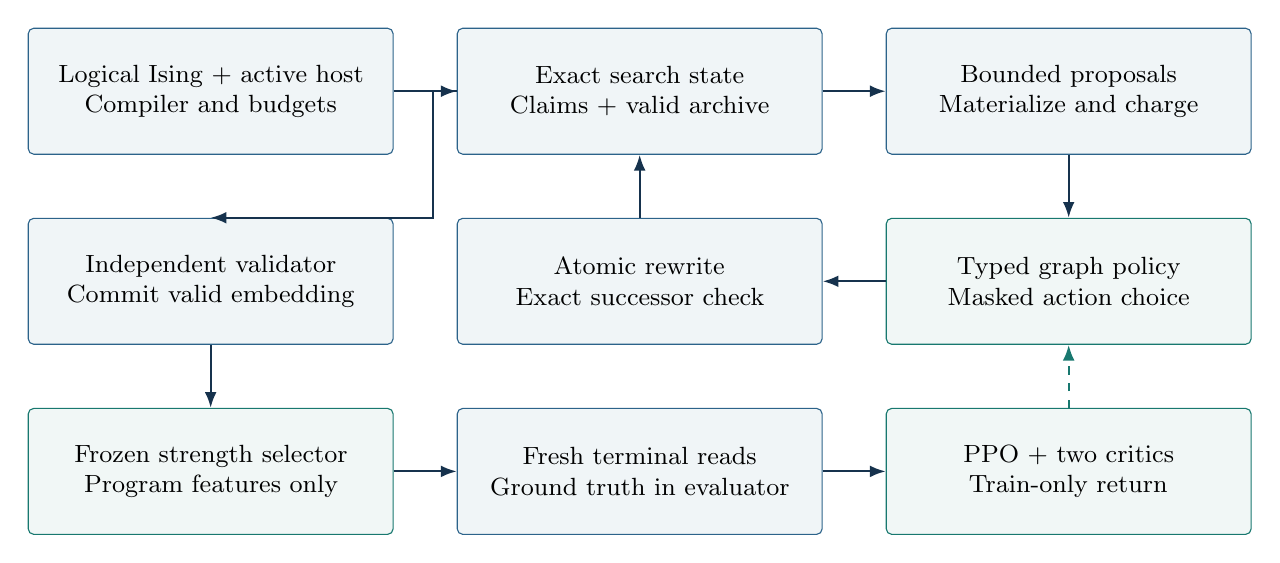
\begin{tikzpicture}[node distance=8mm and 8mm,
box/.style={draw=Blue,fill=Pale,rounded corners=2pt,text width=44mm,minimum height=16mm,align=center,font=\small},
learn/.style={box,draw=Teal,fill=Teal!6},
arr/.style={-{Latex[length=2mm]},thick,draw=Navy}]
\node[box] (in) {Logical Ising + active host\\Compiler and budgets};
\node[box,right=of in] (st) {Exact search state\\Claims + valid archive};
\node[box,right=of st] (gen) {Bounded proposals\\Materialize and charge};
\node[learn,below=of gen] (actor) {Typed graph policy\\Masked action choice};
\node[box,left=of actor] (apply) {Atomic rewrite\\Exact successor check};
\node[box,left=of apply] (gate) {Independent validator\\Commit valid embedding};
\node[learn,below=of gate] (sel) {Frozen strength selector\\Program features only};
\node[box,right=of sel] (eval) {Fresh terminal reads\\Ground truth in evaluator};
\node[learn,right=of eval] (train) {PPO + two critics\\Train-only return};
\draw[arr] (in)--(st);\draw[arr] (st)--(gen);\draw[arr] (gen)--(actor);
\draw[arr] (actor)--(apply);\draw[arr] (apply)--(st);
\draw[arr] (st.west) -- ++(-3mm,0) |- (gate.north);
\draw[arr] (gate)--(sel);\draw[arr] (sel)--(eval);\draw[arr] (eval)--(train);
\draw[arr,dashed,draw=Teal] (train)--(actor);
\end{tikzpicture}
\caption{Registered operating boundary. The search loop uses no true solve probabilities. The evaluator supplies rewards during training and independent scores during testing. The frozen strength selector is shared by all embedders.}
\label{fig:system}
\end{figure}

\subsection{Environment state and semantic observation}
At decision epoch $t$, the environment contains
\begin{equation}
s_t=(I,H,\Omega,\widetilde\phi_t,\mathcal O_t,\mathcal A_t^{\rm inc},m_t,b_t,\mathcal K_t).
\end{equation}
Here $\widetilde\phi_t$ is the relaxed branch-set assignment; $\mathcal O_t(q)$ is the full set of claiming logical variables; $\mathcal A_t^{\rm inc}$ is the valid archive; $m_t$ includes active search mode, revisit/tabu memory and restart counters; $b_t$ is the remaining work vector; and $\mathcal K_t$ is the current materialized candidate batch. The logical and hardware inputs and compiler context are immutable.

The policy receives semantic graph tensors sufficient to describe those objects and their permitted action payloads. Archive program coefficients can be reconstructed from memberships and the deterministic compiler, so duplicating all program bytes into neural features is unnecessary. Hashes, version receipts and random tape identifiers are retained for replay but do not become numeric neural features. Expose an actual priority/rank only when the environment uses that priority to determine subsequent behavior; do not assume arbitrary node IDs are meaningful graph attributes.

Randomized proposal choices are part of a registered transition kernel with fresh exogenous randomness. Full random state is retained for reproducibility; future evaluator randomness is inaccessible to the policy. If persistent random priorities influence later candidate construction, their current semantic values must be observable. A deterministic replay conditioned on a random tape and a stochastic MDP marginalizing that tape are compatible descriptions.

A GNN compresses this structured observation. It is not guaranteed to distinguish every nonisomorphic state or predict every transition. A summary MLP is an intentionally information-limited control. The environment is Markov when it contains all relevant search memory; omitting relevant memory from the controller creates a partially observed approximation and must be disclosed.

\subsection{Controlled overlap invariants}
For $o_t(q)=|\mathcal O_t(q)|$, define
\begin{equation}
X_t=\sum_q(o_t(q)-1)_+,\quad
Q_t^{\rm unique}=|\{q:o_t(q)>0\}|,\quad
Q_t^{\rm claim}=\sum_i|C_i^t|=Q_t^{\rm unique}+X_t.
\end{equation}
A nonempty chain is connected in active hardware. Empty chains are allowed only for unplaced variables in construction mode or a separately registered partial-repair curriculum. All replacements are atomic, so an intermediate implementation buffer may not be published as an environment state.

Initial profiles are O0: $o\le1,X=0$; O1: $o\le2,X\le\lceil0.10B_Q\rceil$; and optional O2: $o\le4,X\le\lceil0.25B_Q\rceil$. In all profiles $Q^{\rm unique}\le B_Q$ and $Q^{\rm claim}\le B_Q+X_{\max}$. O1 is a testable initial choice, not a theorem about the best overlap budget. The unique-qubit search cap may itself prevent useful detours; a later expanded-workspace experiment must distinguish a larger search cap from the unchanged terminal cap.

Sharing a qubit never realizes a logical edge. A contact requires an active physical coupler between distinct endpoint qubits. Contested resources have no exclusive free-capacity credit. Residual-routability features for a chain remove its own claims while keeping all other claims occupied. This is a conservative \emph{feature} graph: absence of a route in it does not prove impossibility in the overlap-enabled action grammar and must not automatically mask a legal repair.

No consistent physical Hamiltonian is assigned to a non-disjoint relaxed state. Program-derived cut or quality features for such a state are marked unavailable, or explicitly tagged as hypothetical local descriptors. The downstream evaluator accepts only independently valid terminal embeddings.

\subsection{A finite, fully bound action grammar}
Every candidate carries a state digest, opcode, affected logical set, old/new branch sets, path-role incidences, structural deltas, exact mask result and work receipt. The actor selects an already materialized successor; it does not emit raw sets for unchecked execution.

{\small\begin{longtable}{@{}P{.20\textwidth}P{.73\textwidth}@{}}
\toprule
Opcode & Payload and semantics\\\midrule\endhead
PLACE & Construction only. Logical variable and complete nonempty connected initial branch set. Placement order is selected through the identity of the variable in the candidate.\\
ROUTE & Construction only. Logical demand, endpoint ownership split, complete path and resulting connected branch sets. Every transit qubit belongs to a named chain. The edge is represented by a contact between distinct endpoints.\\
REWRITE\_ONE & A complete connected replacement for one chain. Grow, shrink, chord addition, boundary relocation and rerouting are attributes of this opcode. It may increase overlap within the envelope.\\
REWRITE\_GROUP & Complete replacements for a logical group, initially $k\in\{2,3,4,8\}$ where size permits. Supports coordinated rerouting and destroy/reconstruct moves. Each successor chain is connected, and unchanged chains remain untouched.\\
REPAIR\_GROUP & Same exact atomic representation as group rewrite, with a conflict/bottleneck-selected group and repair purpose. The repair may move a conflict before eliminating it.\\
RESTART & A bound successor from a registered fresh initialization procedure, materialized and charged during proposal generation. The valid archive survives. Initializer-internal search is bounded and audited.\\
COMMIT & Select one current valid archive entry. Fresh independent validation is mandatory. This is a real terminal action, not an automatic return at first validity.\\
STOP & Explicit ordinary failure when no embedding is returned. Used in construction or a registered voluntary-abandonment experiment; it never disguises an invalid embedding as a valid result.\\
\bottomrule
\end{longtable}}

In the recommended protected-incumbent improvement profile, an archive entry is always available after initialization, and failure-STOP is masked out: stop searching by COMMIT. In construction, STOP is permitted when no archive exists; with a valid archive, termination also uses COMMIT. This avoids learning an unnecessary choice between returning a known valid embedding and returning nothing. The source's voluntary failure action is retained only as a separately named ablation.

\subsection{Candidate construction and diversity}
A fixed generator supplies at most 64 state-changing actions. COMMIT entries (at most eight) and a possible STOP entry are additional, giving a padded maximum of 73. A candidate cap is not a global search guarantee. The generator must expose interacting alternatives, not just many nearly identical shortest routes.

For seeded improvement, an initial per-batch allocation is 16 single-chain proposals, 24 group rewrites (eight each for $k=2,3,4$), eight $k=8$ proposals, 12 conflict/bottleneck repairs and four restarts/restores. If a family is inapplicable, fill from a fixed family order until the common work allowance is exhausted; record the resulting counts. Treat a restore to stored chains as a bound group rewrite, not an uncharged side operation. For construction, separately register quotas for PLACE and ROUTE instead of silently borrowing the improvement grid.

Within a family, mix outcome-blind proposal costs: route length, occupancy pressure, contact multiplicity, free-neighborhood size, and limited randomized edge-cost perturbations. Use fixed coefficients and seeds within an experiment. These costs define proposal diversity, not the reward. Include multiple reconstruction orders for joint moves. A generator may use a frozen deployable proxy only in a separately ablated version shared by controls.

Deduplicate candidates with identical complete successors and update semantics. Different provenance labels should not multiply one successor's policy mass. Do not deduplicate genuinely different persistent-memory updates. Candidate ordering is stable for replay; the actor must be equivariant to a consistent permutation of that order. No quality outcome, planted witness or ground-state reference may determine truncation, masking or candidate ranking.

\subsection{Work must be charged before preference is learned}
Define a work vector with decision count, route expansions, candidate materializations, compiler/validator calls, cut-edge processing, restart work and evaluator reads. Let
\begin{align}
(\mathcal K_t,w_t^{\rm gen})&=G(s_t;b_t^{\rm gen}),\\
b_t^{\rm avail}&=b_t-w_t^{\rm gen},\\
a_t&\sim\pi_\theta(\cdot\mid o_t,\mathcal K_t),\\
b_{t+1}&=b_t^{\rm avail}-w_t^{\rm apply}(a_t).
\end{align}
The generator is interruptible at deterministic work boundaries. It charges attempted and rejected proposals. Budgets for duplicate removal, validity screening, archive admission and optional cut tokens are not free. Every ordinary decision consumes positive decision allowance, ensuring a finite horizon. Masks check whether the remaining \emph{application} cost fits after batch construction.

The complete-system initializer receives its exact coordinatewise remainder before each native call, after reserving the top-level invocation, independent candidate screen, environment bootstrap and terminal policy path. Native counters check a prospective delta before the corresponding operation. An exhausted coordinate therefore terminates explicitly without incrementing beyond its cap. Post-hoc rejection of an initializer that already exceeded a registered operation budget is not a valid implementation of this contract.

Keep a reserved terminal budget for archive replay, COMMIT inference and one final evaluation block. If a normal batch cannot fit, expose a bounded COMMIT-only decision when the archive is nonempty. If it is empty, terminate as a no-valid timeout. Never call softmax with an all-false mask. Wall-clock comparisons reserve enough completion time or return the protected validated object; an external supervisor handles solver timeouts, including calls whose internal timeout is unreliable.

Matching every hardware-specific work coordinate across unrelated solvers is generally impossible. The controlled experiment matches native operation budgets inside a shared environment. External comparison uses a preregistered wall-clock budget on matched hardware plus equal evaluator/QPU resources, and reports operation counts as explanatory metrics. Do not assert exact apples-to-apples route-expansion matching when an external implementation exposes no such counter.

\subsection{Sealed deployment-initializer bank}
PPO in Profile I conditions on successful initialization, but that condition must not be implemented by substituting hand-authored CandidateBank witnesses. Before training, create one target-free initializer-bank plan for each registered training seed. The plan reads public train tasks only and assigns conditional episodes equally over immutable base lineages by canonical round robin. Within a lineage, a seeded cyclic offset chooses the instance. Each episode then receives a finite, deterministic sequence of complete LAC initializer draws. For a registered PPO cell, the bank contains exactly \code{updates $\times$ episodes} snapshots, which is $100\times64=6{,}400$ under the fixed grid. A supervised-only cell consumes no snapshot even though its complete-system interface retains the bank arguments.

Generation executes the planned draw sequence and stops at its first valid initializer. Every rejected draw, failure reason, and work vector remains recorded. A bank cannot be sealed if any conditional episode exhausts its registered draw cap. The plan, snapshots, bank manifest, and access receipt each have immutable v1 schemas. Their identities bind the prepared-v4 public corpus, complete-system configuration, native-extension and Python runtime sources, work context, training seed, episode schedule, and every accepted or rejected draw. Only after the manifest and its out-of-band SHA-256 pin have been authenticated may the training loader open the train target partition and attach rewards. This order keeps initializer selection independent of evaluator targets while making the conditional training distribution exactly replayable.

The bank is a training artifact, not a replacement for complete-system evaluation. Learned and external confirmation start from the full public population before initialization, execute their registered initializer schedules, and retain ordinary initializer failures as zero-utility outcomes. The protected-incumbent property therefore remains conditional, while the publication endpoint remains unconditional.

\subsection{Archive design and publication boundary}
Use eight outcome-blind slots: one protected initial valid embedding and up to seven later independently valid states. Apply deterministic deduplication and FIFO eviction to the seven mutable slots. Store exact memberships, compiler context, resource descriptors and creation order. This prevents losing the initial feasible result, although FIFO can still discard a high-quality unseen candidate. Archive-size and eviction effects are separate from policy effects.

No archive entry contains solver outcomes during search. The actor can use input-derived features to choose COMMIT. Sampling is performed only after final selection in S0. If the system later probes archive quality online, it becomes an evaluator-assisted search algorithm with a charged budget and observation schema; it is a different profile.

A fresh validator reconstructs the full logical domain, active qubit membership, connected programmed chains, disjoint ownership, realization of every logical edge, qubit cap, coefficient sums, exact compiled bytes and range/precision contract. Search caches are not authoritative. A mismatch aborts the affected experiment with its immutable record retained.

\begin{proposition}[Conditional valid-return property]
Assume the independent validator is correct and the only public return path requires its acceptance. Every nonempty embedding returned by the API satisfies the declared graph/program/resource contract, independently of the policy parameters. If Profile I successfully stores a protected admissible initializer and the reserved terminal path executes correctly, later search cannot remove the availability of at least one admissible return.
\end{proposition}
\begin{proof}
The first statement follows directly from the return gate. For the second, induction over actions preserves the protected archive slot; budget exhaustion exposes COMMIT over admissible entries. Neither statement guarantees initialization success, improvement over the initial embedding, or correct operation under an implementation failure.
\end{proof}

In particular, protected feasibility does not guarantee protected \emph{quality}: a learned COMMIT selector can choose a worse archive entry. Detect this by comparing initial versus returned quality on fresh evaluation blocks, and include a return-initial baseline under identical initialization cost.

\subsection{Action-support headroom before RL}
On tiny enumerated cases, distinguish the unrestricted capped optimum $U^*$, the best reachable value in the registered action grammar $U_G^*$ and the deployed policy value $U_\pi$. At the level of optimal expected values,
\begin{equation}
U^*-U_\pi=(U^*-U_G^*)+(U_G^*-U_\pi).
\end{equation}
The first gap is proposal/support limitation; only the second can be removed by a perfect selector under the fixed environment. With stochastic generators, define reachability with their actual support and budgets, not a clairvoyant choice of random tapes.

At larger sizes evaluate candidates with a frozen continuation rule and independent high-read scoring to estimate local ranking headroom. A best-of-$K$ oracle is an upper bound only for that exact candidate set and continuation protocol; it is not a bound over all multi-step policies. Compare neighborhood sizes, contact-diverse routing and non-greedy repair. If expanded candidates have no useful downstream spread, stop scaling the actor and revise the generator or objective regime.

Release Gate 2 uses one selected task per immutable base lineage. For every lineage, it selects the best registered rewrite on one screening read block, then rescores that fixed rewrite and protected COMMIT on independent confirmation blocks. Let $h_i$ be the difference between those confirmed rates. The v6 decision requires the one-sided 95 percent normal lower confidence bound for the mean of the observed $h_i$ values to be at least the registered meaningful effect $\delta=0.02$. Its standard error combines between-lineage variation with the worst-case Bernoulli variance bound for the difference of the two finite-read confirmation rates. It also requires at least half of the sampled rows in every authenticated joint stratum to satisfy $h_i\geq\delta$. A sample with fewer than two eligible lineages fails closed because it cannot estimate between-lineage uncertainty. Support recall, within-support spread and the gap to the frozen broader proposal pool remain separate conjunctive requirements. This is a screening rule for the observed proposal pool, not an inferential claim about the unrestricted optimum $U^*$.
 \section{Theory bridge: what geometry can justify}
\label{theory:bridge}

The useful theory connects a change in an embedding to a change in its programmed energy landscape. It does not identify the best embedding from chain length alone. This section supplies explicit definitions for the cut quantities left implicit in the source architecture and states exactly which conclusions follow. The chain-integrity argument belongs to the sufficient-condition tradition for minor embedding~\cite{choi2008}; the proposition and proof below use the particular coefficient-allocation contract specified here. They are mathematical design support, not a new experimental result or, without a separate literature comparison, a novelty claim.

\subsection{Structural graph, programmed graph, and effective load}
\label{theory:objects}

Fix a structurally valid embedding with disjoint nonempty branch sets $C_i$. Let $E_i^{\mathrm{ch}}$ contain the internal hardware couplers actually programmed ferromagnetically. The induced hardware graph $H[C_i]$ tells us what is available; $(C_i,E_i^{\mathrm{ch}})$ tells us what the physical program uses. These coincide only under the baseline rule that programs every active internal edge.

Write the exact pre-scale Hamiltonian as
\begin{equation}
 E_F(z)=\sum_q \widetilde h_q z_q+
 \sum_{(q,r)\in E_{\mathrm{ext}}}\widetilde J_{qr}z_qz_r
 -F\sum_i\sum_{(q,r)\in E_i^{\mathrm{ch}}}w_{qr}z_qz_r,
 \qquad z_q\in\{-1,+1\},
 \label{theory:physical}
\end{equation}
where $w_{qr}>0$ is a fixed relative chain-edge weight and $w_{qr}=1$ in the initial uniform-strength implementation. The scalar $F$ is selected from the four strengths in the registered objective context. Every external coupler has endpoints in different branch sets. The compiler must satisfy
\[
 \sum_{q\in C_i}\widetilde h_q=h_i,
 \qquad
 \sum_{(q,r)\in R_{ij}}\widetilde J_{qr}=J_{ij}.
\]
Consequently, every chain-consistent state has logical energy plus a state-independent chain offset. The theorem below assumes these exact coefficients, fixed active hardware, and no undeclared physical couplings.

Define an absolute external-load bound at each qubit by
\[
 a_q=|\widetilde h_q|+
       \sum_{r\notin C_i:(q,r)\in E_{\mathrm{ext}}}|\widetilde J_{qr}|,
 \qquad q\in C_i.
\]
For a nonempty proper subset $S\subset C_i$, let
\begin{align}
 D_i(S)&=\sum_{q\in S}a_q,\nonumber\\
 d_i(S)&=\min\{D_i(S),D_i(C_i\setminus S)\},\nonumber\\
 c_i(S)&=\sum_{(q,r)\in\delta_{E_i^{\mathrm{ch}}}(S)}w_{qr},
 \qquad
 m_i(S;F)=F c_i(S)-d_i(S).
 \label{theory:cutquantities}
\end{align}
Here $c_i$ is programmed cut capacity, $d_i$ is a conservative bound on the drive available to pull the two sides apart, and $m_i$ is a sufficient-condition margin. All quantities depend on the actual compiler allocation. Counting nearby hardware edges that are unprogrammed, faulty, or claimed by another chain creates fictitious capacity.

\subsection{A sufficient chain-integrity condition, with proof}
\label{theory:certificate}

\begin{proposition}[Cut-load sufficient condition]
\label{theory:cutproposition}
Under Equation~\eqref{theory:physical}, fix the spins outside $C_i$. For any mixed-spin assignment within $C_i$, let $S$ be its $+1$ side. If $z^{(+)}$ and $z^{(-)}$ replace this chain by its two uniform assignments while leaving the exterior fixed, then
\begin{equation}
 E_F(z)-\min\{E_F(z^{(+)}),E_F(z^{(-)})\}
 \ge 2m_i(S;F).
 \label{theory:repairgap}
\end{equation}
If $m_i(S;F)>0$ for every proper cut of every nonsingleton chain, every global ground state of the physical model is chain-consistent. Under faithful coefficient allocation, its decoded logical state is a logical ground state.
\end{proposition}

\begin{proof}
With the exterior fixed, the effective local field is
$b_q=\widetilde h_q+\sum_{r\notin C_i}\widetilde J_{qr}z_r$, so $|b_q|\le a_q$. Put $B_S=\sum_{q\in S}b_q$ and $B_T=\sum_{q\in C_i\setminus S}b_q$. A mixed chain pays internal energy $2F c_i(S)$ above a uniform chain. Its external-field energy is $B_S-B_T$, whereas the better uniform assignment has external-field energy $-|B_S+B_T|$. Their energy difference is therefore
\[
 2F c_i(S)+B_S-B_T+|B_S+B_T|.
\]
Using $x-y+|x+y|=2\max\{x,-y\}$ and the bounds on $B_S,B_T$ gives a lower bound
$2F c_i(S)-2\min\{D_i(S),D_i(C_i\setminus S)\}$, proving Equation~\eqref{theory:repairgap}. A physical ground state containing a mixed chain would then admit a strictly lower-energy uniform replacement, a contradiction. Among chain-consistent states, faithful programming preserves logical energy ordering, proving the final statement.
\end{proof}

For connected programmed chains, $c_i(S)>0$, and the sufficient threshold is
\[
 F>\tau_{\mathrm{cut}},\qquad
 \tau_{\mathrm{cut}}=\max_i\max_{\varnothing\ne S\subsetneq C_i}
                       \frac{d_i(S)}{c_i(S)}.
\]
Singleton chains have no nontrivial cuts and contribute threshold zero. Strict inequality matters: equality can leave degenerate broken ground states. Failure of this condition establishes only that this certificate is unavailable. Absolute loads ignore cancellation, and the bound can be conservative. It is neither a necessary minimum chain strength nor the strength that maximizes the registered decoded success probability.

A cheaper conservative certificate avoids exhaustive cut-ratio optimization. Let
\[
 A_i=\sum_{q\in C_i}a_q,
 \qquad \kappa_i=\min_{\varnothing\ne S\subsetneq C_i}c_i(S).
\]
Then $d_i(S)\le A_i/2$ and $c_i(S)\ge\kappa_i$, hence
\begin{equation}
 \tau_{\mathrm{cut}}
 \le\max_{i:|C_i|>1}\frac{A_i}{2\kappa_i}.
 \label{theory:mincutcertificate}
\end{equation}
The weighted global minimum cut $\kappa_i$ is computable without enumerating all bipartitions. This bound can certify some chains even when only a small number of cut tokens enter the neural network. It should not be confused with solving the generally more difficult maximum load-to-capacity ratio exactly.

\subsection{Certificates and neural cut tokens have different roles}
\label{theory:tiers}

The registered $K_c=16$ token cap is a representation budget. It does not make a sample of cuts exhaustive. A chain with $n_i$ vertices has $2^{n_i-1}-1$ proper bipartitions modulo complement; a 16-token representation can contain every cut only for very small chains. Keep the proof receipt separate from the token subset.

{\small
\begin{longtable}{@{}p{0.22\textwidth}p{0.72\textwidth}@{}}
\toprule
Evidence tier & Permitted interpretation \\
\midrule
\endhead
All-cut exact & Every proper cut was checked under the stated exact coefficient map. A strictly positive minimum margin certifies the proposition's conclusion. \\
Global-mincut bound & Equation~\eqref{theory:mincutcertificate} was checked with a verified minimum-cut value. Positive clearance is sufficient but can be loose. \\
Sampled cuts & Singleton cuts and selected tree-induced or other deterministic cuts provide explanatory features. Their best and worst observed values describe this pool only. \\
Hypothetical relaxed state & Features describe a declared provisional allocation or an executable disjoint successor. They are marked unavailable wherever overlap prevents a physical program. \\
\bottomrule
\end{longtable}}

For every candidate replacement, recompute the affected valid successor's allocation before computing cut deltas. Record pre/post capacity, load, minimum sampled margin over each registered strength, contact multiplicity, side balance, and certificate tier. Pooling should expose both the worst observed cut and the distribution of observed cuts. Canonicalization and token selection use structure and programmed coefficients only, never terminal labels. A cut with zero capacity and positive load needs a separate indicator; clipping an infinite ratio to a large finite number must preserve that indicator.

\subsection{Autoscaling, quantization, and the limit of the guarantee}
\label{theory:limits}

The handbook's expression $\alpha(F)=\max(1,F/J_{\max})$ describes a special normalization regime. A general ideal compiler must also account for physical fields and all programmed problem couplers. With symmetric field and coupling limits, a simple example is
\[
 a_F=\left[\max\left\{1,
       \frac{\max_q|\widetilde h_q|}{h_{\rm lim}},
       \frac{\max_{q,r}|J^{\mathrm{pre}}_{qr}(F)|}{J_{\rm lim}}
       \right\}\right]^{-1}.
\]
An actual device may impose additional constraints; its versioned compiler remains authoritative. The physical coefficients are scaled by $a_F>0$. Exact common positive scaling preserves ground-state ordering and multiplies the cut margin by $a_F$. It changes the distribution sampled at a fixed device temperature or fixed annealing protocol, however. Raising $F$ can improve chain integrity while reducing the energy scale of the logical problem. The theorem therefore does not justify selecting the largest registered strength.

Quantization is a separate issue. If every physical state's compiled energy differs from its ideal scaled energy by at most $\varepsilon_{\mathrm{all}}$, a sufficient robust repair gap is
\[
 2a_Fm_i(S;F)>2\varepsilon_{\mathrm{all}}.
\]
A coefficient-error $\ell_1$ bound gives a conservative all-state energy-error bound because every Ising monomial has magnitude one. A guarantee checked only on chain-consistent states cannot certify this mixed-versus-uniform comparison. Store the coefficient representation, error model, and certificate assumptions together; otherwise retain the exact-model certificate as a diagnostic only.

Finally, the proposition concerns ground states. A finite-read sampler can produce excited states, and majority decoding can map a broken chain assignment to a correct logical solution. Thus neither a chain-break rate nor a cut certificate is identical to the IF-Q3 success event. The connection to downstream quality must be measured with the registered sampler and decoder.

\subsection{Consequences for the architecture and its ablations}
\label{theory:architecture}

This analysis supports giving the actor access to coefficient allocation, internal cuts, cross-chain contacts, and candidate-specific changes. It does not support hard-coding a monotone preference for more qubits, more edges, lower maximum chain length, or larger $F$. Under uniform same-sign allocation, the total absolute drive on a chain is $|h_i|+\sum_j|J_{ij}|$; geometry redistributes this drive and changes the cut capacities exposed to it. Additional qubits can improve that distribution, or simply create a longer vulnerable chain.

The decisive controlled experiment holds the logical instance, active host, four strengths, compiler, sampler, decoder, and resource cap fixed, then changes one geometric mechanism. Compare a candidate with added useful redundancy to a resource-matched lengthening control; compare distributed contacts to concentrated contacts; and compare cut-aware selection to the same candidate pool scored without cut features. Report margins and decoded quality together. A cut-only surrogate may guide warm starts or serve as an auxiliary target, but the policy is selected by its failure-aware downstream outcome. This preserves the theory's explanatory role without promoting a conservative certificate into an unproved deployment objective.
 \section{Neural architecture: an implementable IF-Core}
\label{sec:model}

\subsection{Architecture decision and learning boundary}

The first trainable model is \textbf{IF-Core}: a width-128 typed graph actor--critic with three local logical/hardware message-passing blocks, two ownership/conflict fusion blocks, and a sparse action--chain factor encoder. It chooses fully materialized macro-actions. It does not generate qubit sets, decide whether an overlap is legal, or certify a physical program. A frozen classical generator supplies the same batch $G(s)$ on shared states to learned and classical selection baselines; their batches naturally diverge when their trajectories visit different states. In particular, a multi-chain replacement is represented as one joint action, not as independent chain scores whose preferred moves may be mutually incompatible.

The first experiment is \emph{improvement from a common feasible seed}. The protected seed remains returnable while the workspace may enter bounded overlap. This makes the learned question concrete: which joint repairs and refinements improve the final downstream objective within the available search budget? Empty-state construction is a separately trained and reported regime. Mixing these regimes in the first training run would obscure whether the policy learned construction, useful escape, or merely the seed generator's distribution.

The architecture intentionally starts below the original PNA--GraphGPS--HGT--gauge stack. Message passing and typed relations already supply the necessary inductive biases~\cite{mpnn2017,hgt2020}. PNA aggregation~\cite{pna2020}, relay attention inspired by GraphGPS~\cite{gps2022}, and gauge-specific representations are subsequent hypotheses. Their additional cost must earn a measurable gain under matched online work, not merely a lower training loss.


\begin{figure}[htbp]
\centering
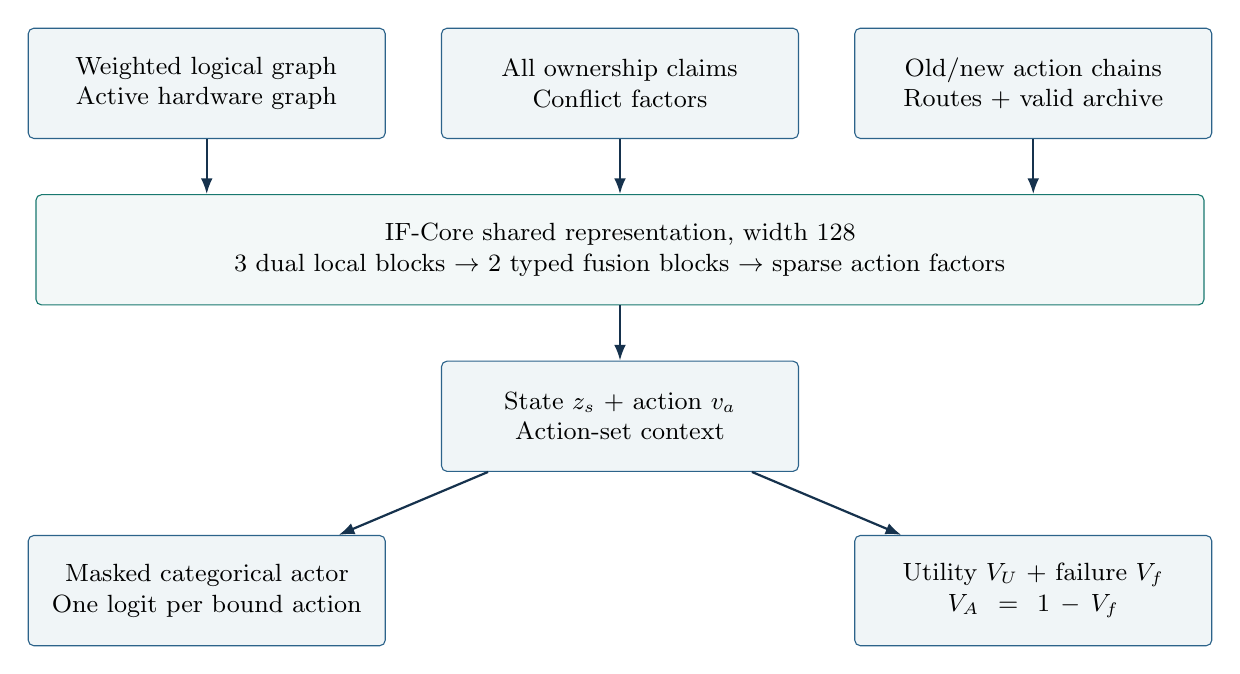
\begin{tikzpicture}[node distance=7mm and 7mm,
box/.style={draw=Blue,fill=Pale,rounded corners=2pt,text width=43mm,minimum height=14mm,align=center,font=\small},
wide/.style={box,text width=146mm,fill=Teal!5,draw=Teal},
arr/.style={-{Latex[length=2mm]},thick,draw=Navy}]
\node[box] (lh) {Weighted logical graph\\Active hardware graph};
\node[box,right=of lh] (own) {All ownership claims\\Conflict factors};
\node[box,right=of own] (payload) {Old/new action chains\\Routes + valid archive};
\node[wide,below=of own] (trunk) {IF-Core shared representation, width 128\\3 dual local blocks $\to$ 2 typed fusion blocks $\to$ sparse action factors};
\node[box,below=of trunk] (state) {State $z_s$ + action $v_a$\\Action-set context};
\node[box,below left=8mm and 7mm of state] (actor) {Masked categorical actor\\One logit per bound action};
\node[box,below right=8mm and 7mm of state] (critic) {Utility $V_U$ + failure $V_f$\\$V_A=1-V_f$};
\draw[arr] (lh.south)--(lh.south|-trunk.north);
\draw[arr] (own)--(trunk);
\draw[arr] (payload.south)--(payload.south|-trunk.north);
\draw[arr] (trunk)--(state);\draw[arr] (state)--(actor);\draw[arr] (state)--(critic);
\end{tikzpicture}
\caption{Concrete initial neural model. Exact masks are supplied by the environment. The separate frozen terminal strength predictor is outside this PPO network. Additional cut or global-attention modules are controlled extensions.}
\label{fig:core}
\end{figure}

\subsection{Observation record, tensorization, and normalization}

The exact environment record contains the weighted logical instance, hardware fault snapshot, all current claims, complete bound candidates, archive payloads, counters, and objective context. The model consumes a deterministic tensorization of that record. These are different objects: serialization can be sufficient to replay a transition, while a finite-dimensional neural embedding and pooled summaries are generally lossy. Neither message passing nor the absence of recurrence proves that the policy observation is Markov sufficient. Hidden generator state must be eliminated or recorded; any remaining observation aliasing is measured and documented.

All integer identifiers are \emph{index keys}, never scalar features. Logical and hardware labels, candidate hashes, generator seeds, program digests, file names, dataset families, planted partitions, planted spin assignments, optimum energies, sampled success counts, and downstream labels do not enter learned feature channels. Counters and remaining budgets do enter as numerical values when they affect decisions. Immutable compiler, decoder, sampler, and normalization versions are bound by the experiment registry. A version mismatch rejects a batch; it is not mapped to an unseen trainable ID embedding.

For each scalar slot store a value and a knownness bit. With slots \(u_1,\ldots,u_D\), the input is
\[
 x=\bigl[\widetilde u_1,\ldots,\widetilde u_D,
         m_1,\ldots,m_D\bigr]\in\mathbb R^{2D},
 \qquad \widetilde u_j=0\ \text{when }m_j=0.
\]
An observed zero has \(m_j=1\). Padding is a separate node/action mask. Binary quantities also retain a knownness bit so that absent calibration and a measured zero are distinguishable. Fit continuous normalizers using the training split only and freeze them for development, test, and deployment. For coefficient-like values use a signed logarithmic map
\[
 T_c(x)=\operatorname{sgn}(x)\log(1+|x|/c_{\rm train}),
 \qquad c_{\rm train}>0,
\]
with a recorded train-set scale. Counts use \(\log(1+x)\); bounded fractions remain in \([0,1]\). Use distinct normalizers for logically different units. Avoid per-instance unit normalization that erases the physical difference between weak and strong instances. Keep both signed \(h,J\) and magnitude channels; also expose absolute coefficient scales and hardware ranges in the global context. All features below are available before the action is selected.

\subsection{Exact core feature schema}

The following schemas fix the first implementation. Slots are one-based. Their dimensions count knownness bits but exclude indexing tensors. Combinatorial fractions over an empty set are zero with knownness one; physically undefined ratios use knownness zero. A quantity that has no physical interpretation uses \(m=0\), rather than a fabricated zero.

\begin{longtable}{@{}p{0.18\textwidth}p{0.10\textwidth}p{0.66\textwidth}@{}}
\toprule
Object & Width & Scalar slots before knownness bits \\
\midrule
\endfirsthead
\toprule Object & Width & Scalar slots before knownness bits \\
\midrule
\endhead
Logical node \(L_i\) & 40 &
1 signed \(h_i\); 2 \(|h_i|\); 3 degree; 4 sum of incident \(|J|\); 5 maximum incident \(|J|\); 6 signed incident sum; 7 positive-coupler fraction; 8 nonempty-chain flag; 9 chain size; 10 programmed chain-edge count; 11 induced active edge count; 12 realized incident-demand fraction; 13 number of contested claims; 14 maximum occupancy on the chain; 15 chain boundary edge count; 16 distinct free neighboring qubits; 17 age since this chain changed; 18 remaining tabu duration; 19 physical distance to the nearest unrealized neighboring chain; 20 current connectedness flag. \\
\addlinespace
Hardware node \(H_q\) & 36 &
1 active flag; 2 active degree; 3 nominal degree; 4 occupancy; 5 contested flag; 6 free-neighbor fraction; 7 occupied-neighbor fraction; 8 faulty-neighbor fraction; 9 distinct neighboring claimants; 10 signed compiled bias; 11 magnitude of compiled bias; 12 maximum incident compiled-coupler magnitude; 13 measured bias offset; 14 bias noise standard deviation; 15 readout error rate; 16 time since last occupancy change; 17 distance to an active free vertex; 18 local active two-hop vertex count. \\
\addlinespace
Logical edge \((i,j)\) & 12 &
1 signed \(J_{ij}\); 2 \(|J_{ij}|\); 3 realized flag; 4 number of active physical inter-chain edges; 5 shortest active distance between the branch sets; 6 age of an unrealized demand. \\
\addlinespace
Hardware edge \((q,r)\) & 20 &
1 active flag; 2 shared-claimant count; 3 distinct endpoint-claimant pair count; 4 programmed chain-edge flag; 5 programmed logical-coupler flag; 6 signed compiled coupling; 7 compiled-coupling magnitude; 8 measured coupling offset; 9 coupling noise standard deviation; 10 fraction of endpoint claims involved in overlap. \\
\addlinespace
Claim \((i,q)\) & 12 &
1 claim age; 2 contested flag; 3 number of chain-internal active neighbors; 4 chain boundary flag; 5 chain articulation flag; 6 number of realized incident logical demands attached at \(q\). \\
\addlinespace
Conflict factor \(X_q\) & 8 &
1 occupancy minus one; 2 conflict age; 3 number of distinct neighboring claimants; 4 number of adjacent active free vertices. \\
\bottomrule
\end{longtable}

Define active distance using a capped breadth-first search with a registered radius. A distance not found inside the cap is marked unknown, and the reachability/cap outcome is retained in the exact record; zero is never used to mean ``far away.'' Nominal hardware is retained when available: disabled vertices and edges are observable with active flag zero, while route materialization uses only active support. If only an active host is supplied, nominal-degree and fault-neighborhood values are missing. Never infer a calibration feature from labels or fitted test residuals.

Compiled-coefficient channels refer to a deterministic, currently valid physical program at the registered reference strength \(F_1\). They are missing in an overlapping or otherwise nonprogrammable workspace. Counts such as chain size, overlap, and active boundary remain defined there. A hypothetical local load may be useful in a later extension, but must use separate feature slots with an explicit hypothetical flag; it cannot populate a ``programmed physical bias'' slot. Singleton articulation flags are false by the registered convention. Expensive statistics, including articulation and distance, are charged to feature construction and cached only when their dependency keys match.

The 32 scalar \textbf{global slots}, hence width 64, are: (1) logical vertex count; (2) logical edge count; (3) active hardware vertices; (4) active hardware edges; (5) qubit cap; (6) currently claimed union size; (7) total excess occupancy; (8) total unrealized demands; (9) remaining decision fraction; (10) remaining deterministic work fraction; (11) remaining restarts; (12) current archive size; (13) workspace-valid flag; (14) protected-seed-available flag; (15) absolute logical RMS coefficient scale; (16) maximum logical coefficient magnitude; (17--20) the four registered chain strengths; (21) hardware field range; (22) hardware coupler range; (23) current compile rescaling factor; (24) improvement-mode flag; (25--32) the remaining fractions for route expansions, candidate materializations, compiler calls, validator calls, cut-edge visits, initialization/restart work, reserved terminal work, and feature/inference work respectively. A nonbinding cap has knownness zero; a binding exhausted cap is known zero. Each cap and unit is fixed in the registry. This budget vector prevents two states with different applicable work constraints from being aliased into one generic remaining-work fraction. Slot 15 is exactly $S_I$ defined in Section~\ref{sec:objective}, including zero fields in its denominator and its registered numerical floor. Slot 23 is missing when the workspace cannot be compiled. Temperature, anneal schedule, quantization, and noise model are fixed within this first registry; if any varies, a versioned context extension must expose its deployment-available values before retraining.

\subsection{Ownership and action tensors preserve relational identity}

For a batch of \(b\) observations, concatenate disjoint graphs and keep a batch-index vector for each node type. Let \(n,m\) denote the total logical and nominal hardware vertices; \(e_L,e_H\) are directed edge counts, with both orientations stored. The core schema therefore has 120 named scalar slots across its eight object types, encoded as 240 value/knownness channels distributed across types, plus the eight opcode indicators. This is a schema count, not the input size of a particular graph: chain factors, routes, archive entries, and optional cuts add the explicitly listed relational features. The feature arrays are
\[
 X_L\!:\!n\times40,\quad X_H\!:\!m\times36,\quad
 X_{E_L}\!:\!e_L\times12,\quad X_{E_H}\!:\!e_H\times20,
 \quad X_g\!:\!b\times64.
\]
Index arrays \(I_L\in\mathbb N^{2\times e_L}\) and \(I_H\in\mathbb N^{2\times e_H}\) carry endpoints. The ownership index \(I_O\in\mathbb N^{2\times M}\), where \(M=\sum_i|C_i|\), contains \emph{every} pair \((i,q)\), with \(X_O\in\mathbb R^{M\times12}\). A contested qubit owned by three chains contributes three claims. A single owner ID or binary occupancy would lose precisely the information needed for joint repair.

Create one conflict factor per contested qubit and connect it to that qubit and to every claimant logical node. A chain-pair conflict is consequently not reduced to whichever claimant was inserted first. Indexing tensors are int64; feature tensors are float32 at the input boundary; masks are Boolean. Sorting or hashing is permitted for canonical serialization and duplicate removal, not as a semantic neural feature.

There are at most 64 state-changing candidates, eight archive commits, and one STOP candidate: \(A\le73\) per observation. The opcode one-hot has width eight, ordered as \code{PLACE}, \code{ROUTE}, \code{REWRITE\_ONE}, \code{REWRITE\_GROUP}, \code{REPAIR\_GROUP}, \code{RESTART}, \code{COMMIT}, \code{STOP}. PLACE and ROUTE are disabled in the initial improvement regime. Group rewrites use registered sizes from \(\{2,3,4,8\}\). Grow and shrink are attributes of REWRITE\_ONE. The same atomic action may improve or worsen immediate structural summaries within the permitted workspace constraints.

Each action has 24 scalar descriptor slots, knownness bits, and its opcode, for \(X_A\in\mathbb R^{A\times56}\): (1) affected chains; (2) old claim incidences; (3) new claim incidences; (4) added claims; (5) removed claims; (6) union-size delta; (7) maximum-chain-length delta; (8) total-overlap delta; (9) contested-vertex delta; (10) unrealized-demand delta; (11) resulting maximum occupancy; (12) resulting structural-validity flag; (13) resulting qubit-cap slack; (14) exact charged proposal work; (15) bound transition-work upper bound; (16) maximum route length; (17) mean route length; (18) affected-boundary-edge delta; (19) affected-free-neighbor delta; (20) remaining restart count after action; (21) referenced archive age; (22) referenced archive union size; (23) restores an archived structure flag; (24) changes the workspace flag. Counterfactual structural features come from the already materialized successor, with no downstream sampling. Commit-only and STOP-inapplicable values are missing.

\textbf{The descriptors supplement complete action incidence; they do not replace it.} For every changed logical chain create factors \(B_{a,i}^{\rm old}\) and \(B_{a,i}^{\rm new}\), connected to action \(a\), logical node \(i\), and all qubits in the corresponding old or new branch set. Each factor has eight scalar slots (width 16): phase-is-new, branch-set size, induced active edge count, programmed chain-edge count, boundary edge count, contested-claim count, connectedness, and changed-from-old flag. Set membership is unordered. When a bound payload contains an ordered route, attach a separate route factor and route--qubit incidences carrying normalized position, start flag, end flag, and logical-attachment flag (four values plus four knownness bits, width eight). Do not assign artificial positions to an unordered branch set.

For programmed chain edges and inter-chain realizations, retain factor-to-hardware-edge indices, with relation labels distinguishing old chain edges, new chain edges, old realization, and new realization. Preserve the logical-edge reference for every realization. A route transit vertex always has an explicitly identified claimant. Thus two group actions that touch the same union of qubits but assign those qubits to different chains receive different incidence graphs. Store complete deterministic program payloads in the environment record, including all coefficient vectors and compiler context; program bytes must be reconstructible independently of the policy. Digests verify identity but neither replace those payloads nor become floating-point inputs. The neural encoder still need not be injective over these records.

\subsection{Forward computation and prediction heads}

Project each node or factor type independently to width \(d=128\), using a linear map, SiLU, and LayerNorm. Project edge and incidence feature vectors to width 32. The logical and hardware encoders have separate weights. Each of three local blocks uses a message MLP \(288\!\to\!128\!\to\!128\), because its concatenation contains two width-128 nodes and a width-32 edge:
\[
 m_{uv}^{(r)}=\operatorname{MLP}^{(r)}_m
 [z_u,z_v,e_{uv}],\qquad
 a_v=\bigl[\operatorname{mean}_{u}m_{uv},
             \operatorname{max}_{u}m_{uv}\bigr]\in\mathbb R^{256},
\]
\[
 z_v^+=\operatorname{LN}\!\left(z_v+
 \operatorname{MLP}^{(r)}_u[z_v,a_v]\right),
 \quad \operatorname{MLP}^{(r)}_u:384\to256\to128.
\]
Empty-neighborhood aggregates are zero. Degree is an explicit feature, so mean aggregation does not silently erase neighborhood cardinality. The two subsequent fusion blocks use relation-specific message maps and the same mean/max update for logical-to-hardware ownership, its reverse, claimant-to-conflict, conflict-to-claimant, conflict-to-qubit, and reverse relations. Sum relation contributions before the residual update. This is a sparse typed MPNN; it does not require full Transformer attention to express ownership. Before action pooling, contextualize each logical/hardware edge with a \(288\to64\to32\) MLP applied to the endpoint-embedding sum (128), their elementwise absolute difference (128), and the projected raw edge features (32). This preserves an endpoint-dependent edge representation while remaining insensitive to reversing an undirected edge.

Encode each action-chain factor using its projected descriptor (128), logical-node embedding (128), membership-node mean/max (256), programmed-hardware-edge mean/max (64), and realized-logical-edge mean/max (64). The last two use the corresponding width-32 edge embeddings. A shared \(640\to256\to128\) MLP produces the factor embedding; old/new phases remain separate factors. For ordered routes, concatenate each hardware-node embedding with its width-32 projected positional incidence features and project \(160\to128\). Apply a shared one-dimensional gated convolution with kernel three and two layers, width 128. Concatenate sequence mean, maximum, first, and last embeddings and project \(512\to128\) to obtain a route factor; total route work is linear in recorded route incidences. Build an action vector from its projected descriptor (128), old/new chain-factor mean/max (256), route-factor mean/max (256), touched-conflict mean/max (256), and referenced archive token (128), then project \(1024\to256\to128\). Absent relation pools are zero, with presence recoverable from the typed incidences and descriptor masks. RESTART proposals bind their materialized initialization payload before scoring. COMMIT actions refer to the corresponding archived structure. Node-level edge messages distinguish endpoint assignments even where pooled summaries collide; no injectivity guarantee is assumed.

Pool current logical, hardware, and conflict embeddings with type-specific mean and maximum pooling. Empty types contribute zeros and their count is retained. Include the archive representation described below. The six current-type pools contribute 768 channels, the archive summary contributes 128, and global context contributes 64. A \(960\to256\to128\) projection maps this result to \(z_s\in\mathbb R^{128}\). Let \(v_a\in\mathbb R^{128}\) denote the action representation. Introduce a permutation-invariant action-set summary
\[
 c_{\mathcal A}=\operatorname{MLP}_{\rm set}
 \left[\operatorname{mean}_{a\in\mathcal A_{\rm live}}v_a,
       \operatorname{max}_{a\in\mathcal A_{\rm live}}v_a\right]
 \in\mathbb R^{128}.
\]
Only real, admissible candidates enter this summary; padded rows are excluded. The actor tower is \(512\to256\to128\to1\):
\[
 \ell_a=\operatorname{MLP}_\pi
 [v_a,z_s,c_{\mathcal A},v_a\odot z_s],\qquad
 \pi_\theta(a\mid o,\mathcal A)=
 \frac{M_a\exp(\ell_a-\ell_{\max})}
 {\sum_j M_j\exp(\ell_j-\ell_{\max})}.
\]
Masking is implemented as a logit operation before normalization. The environment guarantees a nonempty support; an all-false mask is an implementation error with a recorded fallback, not a distribution on invalid actions. Candidate permutations merely permute logits if all associated indices move with them. This is tensor-order equivariance; it does not imply invariance to changing a generator's canonical tie-break process.

Separate towers read \([z_s,c_{\mathcal A}]\in\mathbb R^{256}\). The utility critic \(V_U\), with hidden widths \(128,64\), predicts expected \emph{unshaped terminal utility}, including fallback behavior. Its output is linear so shaping corrections need not force a sigmoid range. The failure critic \(V_f\) has the same widths and a sigmoid output, predicting the policy's probability of returning no admissible embedding; define \(V_A=1-V_f\). Conditional on successful initialization and ordinary execution, the protected feasible seed makes failure identically zero in improvement mode. The unconditional system still includes initializer failures. Its failure critic is therefore a monitoring/constraint head, not evidence of learning construction feasibility. Each tower receives only the current deployment-available observation and candidates. Terminal outcomes appear as stopped-gradient targets after rollout; they never enter the trunk as input features. Actor and critics share the trunk initially; a split trunk is justified only by measured interference.

\subsection{Archive representation and separate strength predictor}

A mutable archive influences future commits and therefore cannot be invisible to the critic. The default bound is eight entries, including the protected seed. For each entry create an archive token and a factor for each archived chain. Include archive age, protected status, admissibility, qubit use, and chain-length summaries as five scalars with knownness bits (width ten). Attach complete archived chain membership and programmed-edge/realization incidences to hardware nodes/edges, using archive-specific relation types. Do not reuse current ownership in place of archived ownership. The same chain-factor encoder can share weights while preserving its phase/archive type. Pool entries with mean/max operations to a width-128 archive summary; append this summary to state pooling. The full membership cost is paid explicitly. An archive-summary-only model is an ablation with partial observation, not a lossless optimization.

The separately pretrained \(q_\psi\) is a \textbf{terminal chain-strength selector}, not the PPO critic and not an oracle for invalid workspace states. It receives a valid program-ready embedding bundle and its four compiled programs, with only deployment-available instance, program, strength, and hardware context. A shared program graph encoder, conditioned on the corresponding scalar strength, emits
\[
 q_\psi(\Pi)=
 (\widehat p_\psi(\Pi_{F_1}),\ldots,
  \widehat p_\psi(\Pi_{F_4}))\in[0,1]^4.
\]
A concrete first selector uses separate copies of the width-128 three-local/two-ownership-fusion graph trunk, with weights shared across strengths but not shared with PPO. Omit action, route, conflict and archive modules. For strength $F_j$, populate physical coefficient channels with that actual compiled program, pool logical and hardware nodes by mean/max (512 channels), and concatenate global context (64), a four-dimensional strength-index one-hot, and two scalars $F_j$ and $a_{\phi,F_j}$ (582 total). An MLP $582\to128\to64\to1$ with sigmoid emits the strength response. All four passes share weights; cache only strength-independent features. This is a fully specified initial predictor rather than an unspecified oracle. There are exactly four probability outputs and no leaked optimum-energy, success-count, or evaluator-receipt inputs. For example, train with aggregated binomial negative log-likelihood using training-only \((K_F,N_F)\) labels; cap or register weighting so heavily sampled items do not accidentally dominate. Fit any calibration on a reserved selector-calibration subpartition of training, disjoint from the RL architecture-selection development set. Freeze all selector weights, normalizers, calibration, and tie rules before PPO collection, then choose the terminal strength using its registered four-way selection rule. Evaluation labels must come from the independent evaluator specified elsewhere in this document. Predicted values are not substituted for final measured utility. No gradient passes from PPO through \(q_\psi\), and its predicted scores are not appended to intermediate action features in IF-Core. A scorer-guided proposal policy would be a separately costed, separately ablated method.

\subsection{Optional cut tokens and physical interpretation}

Add cut tokens only after IF-Core passes the mechanism and benchmark gates. A token references chain \(i\), an explicitly stored proper side \(S\), phase (current/old/new/archive), and strength index. At most 16 cuts per affected chain and phase are sampled by a frozen deterministic procedure. Its twelve scalar slots (width 24) are: strength; side-size fraction; boundary-edge count; programmed cut capacity; smaller-side absolute drive bound; capped drive/capacity ratio; capacity-zero flag; drive-zero flag; exhaustive-enumeration flag; physical-program-valid flag; smaller-side attachment load; and structurally determined violation flag. The cut-side membership is retained in index tensors. Capacity and drive are masked missing without a valid applicable physical program. They must not treat multiply claimed qubits as independent physical capacity.

The exact drive/capacity convention comes from the registered programming theorem and compiler, not a new neural definition. A finite collection of sampled cuts is a diagnostic feature set. It supplies neither the minimum over every proper cut nor a chain-integrity certificate. ``Exhaustive'' is true only when every complement-distinct proper cut was checked. Any certificate auxiliary loss uses only exact or independently certified targets and an explicit applicability mask. The ablation must separate a richer cut representation from adding a certificate loss.

\subsection{Training mechanics, cost, and model ladder}

Use dropout zero in the actor trunk, factor encoder, and all PPO heads, including any pretrained components reused there. LayerNorm is deterministic and avoids train/evaluation BatchNorm drift. A rollout stores old logits or chosen-action log probabilities, exact masks, candidate payloads, feature-normalizer version, and observation reconstruction keys. During PPO epochs, reconstruct the \emph{same} action batch and observation; never rerun a randomized or updated proposal generator to recompute an importance ratio. The proposal generator does not learn during PPO. Changing quotas, generator weights, or strength-selector weights requires a new collection phase and experiment version.

Let \(M\) be current claims, \(R\) all action old/new/route/edge incidences, \(B\) all archived memberships and edge incidences, and \(C\) all optional cut memberships. For fixed depth and width, sparse forward cost is linear in
\[
 n+m+e_L+e_H+M+R+B+C+A
\]
up to width-dependent message-MLP factors (typically \(O(d^2)\)). Activation memory has the corresponding \(O(d)\) factor. The bound \(A\le73\) does \emph{not} bound \(R\): a few long group replacements can dominate inference. Register maximum group size, route/chain payload lengths, total incidence count, and batch memory; reject or truncate proposals by the frozen rule before they reach the actor. Account separately for candidate construction, successor feature extraction, cut generation, compiler calls, exact validation, archive maintenance, and neural inference. No dense \(m\times m\) hardware attention is used. A later fixed-size relay module adds \(O(mrd)\) attention work for \(r\) relays, plus its projections; report the added cost.

\begin{center}
\small
\begin{tabularx}{\textwidth}{@{}p{0.16\textwidth}XX@{}}
\toprule
Model & Added mechanism & Question answered \\
\midrule
IF-MLP & Shared MLP on the same exact scalar state/action descriptors and action-set pooling & Are expensive graph encoders necessary beyond engineered observations? \\
IF-Dual & Three separate local logical/hardware MPNNs plus phase-aware action-chain pooling & Does graph structure improve action selection? \\
IF-Core & Two typed ownership/conflict fusion blocks over IF-Dual & Does explicit cross-graph and multi-claimant information improve joint repair? \\
Core+cuts & Applicable sampled cut tokens; certificate head as a separate toggle & Does cut information add value beyond overlap and topology? \\
Core+relay & Fixed-count sparse relay communication & Does long-range communication repay its inference cost? \\
Gauge mode & Separately specified invariant/equivariant channels in a sign-symmetric objective context & Does the symmetry help beyond simple gauge augmentation? \\
\bottomrule
\end{tabularx}
\end{center}

All models share the generator, quotas, exact masking rules, seed structures, archive rules, terminal selector, evaluator, and budgets. On a shared state their candidate support is identical; different trajectories need not visit identical batches. Include width/parameter-matched controls when attributing a representation gain. For IF-Core specifically, compare multi-chain versus one-chain support, overlap allowed versus forbidden, full claimants versus binary occupancy, action-chain incidence versus union-only pooling, signs plus magnitudes versus magnitudes alone, and frozen uniform/classical selection versus learned selection. Disabling multi-chain support changes the search space, so report it as a search-space ablation rather than solely a network ablation. Gauge augmentation is the first inexpensive symmetry control; exact gauge invariance is not claimed when device calibration, quantization, decoder ties, or proposal rules break the required symmetry. Select the smallest model with reproducible terminal gains and acceptable runtime. A deeper architecture is a candidate to test, not the project's default conclusion.
 \section{Reinforcement learning and optimization contract}
\label{sec:rl-training}

\subsection{What the first policy is trained to do}

The recommended first learning experiment is \emph{embedding improvement}: every method receives
the same independently valid starting embedding, the same active hardware graph, and the same
remaining search budget. The environment retains that starting program as a protected incumbent.
The actor chooses structural rewrites, temporary overlap, repair, and eventual commitment. This
experiment isolates whether learned sequential decisions improve quality beyond the shared
initialization and proposal machinery. The starting embedding is a feasible fallback, not an action
label or a claim of optimal quality. Its generation time is reported separately and included in the common end-to-end budget. Define $A_{\rm init}$ as initializer success. Post-initialization PPO samples the conditional population $A_{\rm init}=1$; whole-system evaluation also retains $A_{\rm init}=0$ cases with zero utility.

Empty-state construction is a second experiment with a separate initial-state distribution. It adds
placement, ordering, and the possibility that no valid incumbent is ever found. A construction result
must not be inferred from an improvement result. With a protected valid incumbent and a mandatory
valid fallback, the improvement environment returns a valid embedding on every scientifically
completed episode. Conditional on $A_{\rm init}=1$, its failure constraint is therefore inactive by construction; meaningful
feasibility learning occurs in construction or explicitly registered repair populations without
such a fallback. Integrity and evaluator failures remain experiment errors, not ordinary search
failures.

The network is an actor--critic policy because its choices change future states and action supports,
and its parameters are updated from complete trajectory outcomes. A pretrained candidate ranker
used greedily without those trajectory updates is a supervised controller. Both are necessary
controls, but they answer different questions.

\subsection{IF-Q3 terminal reward and the information boundary}
\label{sec:rl-q3}

Let the four registered strengths be \(\mathcal F=\{F_1,F_2,F_3,F_4\}\). A pretrained terminal
program predictor \(q_\psi(\Pi_\phi,F)\) selects
\begin{equation}
 F_\psi(\phi)=\mathop{\arg\max}_{F\in\mathcal F}q_\psi(\Pi_\phi,F),
 \label{eq:rl-strength-selector}
\end{equation}
with a fixed tie rule. The selector consumes only deployable program features. Its weights,
preprocessing, input schema, and four-strength order are frozen before the RL run and are shared by
all compared methods. It has no PPO gradient and does not inspect final evaluator reads. Its offline
training uses separately generated per-strength count labels and training lineages. The selector is
not the policy's continuation critic: it predicts the quality of a specified complete program,
whereas a continuation critic averages over future search decisions.

For a committed admissible embedding \(\phi\), an independent evaluator obtains \(N_{\rm est}\)
registered reads at \(F_\psi(\phi)\), decodes them, and records the integer hit count
\begin{equation}
 K_{\rm est}=\sum_{r=1}^{N_{\rm est}}
 \mathbf 1\!\left\{E_I(D_\phi(z_r))\le E_0(I)+\varepsilon_I\right\}.
 \label{eq:rl-terminal-count}
\end{equation}
The trusted benchmark evaluator may know certified \(E_0\); the deployed actor and selector do not
need it. In particular, deployment never chooses a strength by comparing ground-state hit counts.
Only the selected-strength evaluation is required online by this protocol. Evaluating all four
strengths is a separately charged diagnostic or offline labeling operation.

For a trajectory with \(T\) actions, use transition indices \(t=0,\ldots,T-1\). Let \(A_T\)
indicate an independently admissible returned program. Define
\begin{equation}
 R_T=A_T\frac{K_{\rm est}}{N_{\rm est}},\qquad C_T=1-A_T,
 \label{eq:rl-terminal-outcome}
\end{equation}
with \(R_T=0\) on ordinary no-valid-return failure. Base rewards and costs are zero except that
\(r_{T-1}=R_T\) and \(c_{T-1}=C_T\). Invalid outputs are never sampled or published. Missing
reads, a broken certificate, or an evaluator exception invalidate the affected run rather than
entering the denominator as a zero-hit read.

If evaluation reads follow the registered distribution and are independent of the decisions that
selected the program, then, conditional on the complete terminal program,
\begin{equation}
 \E[R_T\mid\phi,A_T=1]
 =p_{\mathrm{solve}}^{\rm MV}(\phi,F_\psi(\phi)).
 \label{eq:rl-reward-unbiased}
\end{equation}
Independent read blocks support ordinary binomial uncertainty calculations. If a provider uses
correlated reads, retain its block structure and estimate uncertainty at that level; a binomial
interval is not automatically justified. Fresh terminal streams are distinct from selector training,
counterfactual labeling, and final confirmation streams. Reusing one fixed reward tape across many
adaptive policy updates can allow overfitting to that tape even when no individual outcome appears
in the observation.

\subsection{Decision time, macro duration, and work budgets}

The policy acts at macro-decision epochs. One route replacement can require more native work than
another; this is compatible with a finite-horizon decision-epoch MDP when the state contains the
remaining registered budgets. An explicit duration-based formulation is semi-Markov, but the target
here remains undiscounted terminal utility: \(\gamma=1\). Introducing \(\gamma^{\Delta w}<1\)
would prefer earlier reward and would change that target.

Every proposed batch costs work before an action is sampled. If \(b_t^-\) is the budget before
proposal generation, define
\begin{align}
 (\mathcal K_t,c_t^{\rm prop})&=G(s_t^-;b_t^-), &
 b_t&=b_t^- -c_t^{\rm prop},\\
 b_{t+1}^-&=b_t-c_t^{\rm apply}(a_t). &&
 \label{eq:rl-budget-accounting}
\end{align}
All quantities are vectors when decisions, route expansions, compiler calls, and restarts have
separate caps. The actor observes the post-proposal available budget \(b_t\). The generator charges
unsuccessful route searches, rejected candidates, deduplication, successor construction, and any
cut computations. The apply cost cannot retrospectively erase those charges. Tensorization and
inference are also timed; native work units alone do not establish equal wall-clock cost.

Generation must stop before its allotted work is exhausted. Every nonterminal decision consumes a
positive decision allowance, and publication validation has a reserved allowance or a separately
declared terminal budget. A budget-ending transition is a real terminal transition. A forced
commit-only decision is made over eligible incumbents when one exists; otherwise construction
terminates as an ordinary no-valid timeout. Collector boundaries used for batching must not be
mistaken for such environment timeouts.

\subsection{Policy distribution and exact likelihood replay}

The first implementation uses one categorical distribution over fully bound candidate records,
including commit candidates. For stored observation \(o_t\), batch \(\mathcal K_t\), and exact mask
\(M_t\),
\begin{equation}
 \pi_\theta(a\mid o_t,\mathcal K_t,M_t)=
 \frac{M_t(a)\exp\ell_\theta(o_t,a)}
 {\sum_{b\in\mathcal K_t}M_t(b)\exp\ell_\theta(o_t,b)}.
 \label{eq:rl-flat-policy}
\end{equation}
The implementation uses masked log-softmax. It handles terminal fallback before invoking the actor
and never evaluates an all-false support. Exact invalid-action masking belongs to the environment;
the network cannot turn a heuristic preference into a hard mask~\cite{masking2020}.

Proposal generation is frozen during the complete experiment version. In particular, rollout
sampling and PPO updates use the same saved candidate identities, payloads, order, and mask.
Candidates are not regenerated under the current model. If a future extension learns the proposal
distribution \(g_\omega\), its joint policy becomes
\begin{equation}
 \pi_{\theta,\omega}(\mathcal K,a\mid s)
 =g_\omega(\mathcal K\mid s)\pi_\theta(a\mid s,\mathcal K).
\end{equation}
Updating \(\omega\) while omitting this first factor from the likelihood ratio is not the present
algorithm. Learning a neighborhood generator should therefore be a later, separately specified
module.

\textbf{All dropout probabilities are zero during RL collection and update.} Normalization
statistics and stochastic graph encodings are frozen or deterministic. Otherwise fresh dropout
masks can change the probability of a stored action before any parameter update. The replay record
contains the observation or reconstructible semantic tensors, exact action support, sampled ID,
old log probability, old critic predictions, terminal flags, costs, rewards, and version digests.
Before the first optimizer step, reevaluating each stored action must reproduce its old log
probability and give a likelihood ratio of one within the declared numerical tolerance.

\subsection{Two critics with explicit meanings}

The required heads are
\begin{equation}
 V_U^\pi(s)=\E_\pi[R_T\mid s],\qquad
 V_f^\pi(s)=\Pr_\pi(A_T=0\mid s).
 \label{eq:rl-critics}
\end{equation}
The utility head is trained directly. The failure head uses a sigmoid output. For every ordinary
outcome, the implied valid-return probability is exactly \(V_A=1-V_f\); a third independently
fitted validity head is unnecessary. Neither head is an optimal value oracle. Both depend on the
current policy, remaining budget, and initial-state population.

Complete-episode Monte Carlo targets are \(R_T\) and \(C_T\) for each preceding state in that
episode. A straightforward critic loss is
\begin{equation}
 \mathcal L_V=
 c_U\,\operatorname{MSE}(V_U,R_T)
 +c_f\,\operatorname{BCE}(V_f,C_T).
 \label{eq:rl-value-loss}
\end{equation}
MSE targets the conditional mean of the raw utility. The observed \(K/N\) remains a noisy sample
mean, not an exact probability label. Optional structural prediction losses have separate weights
and a no-auxiliary control; their outputs cannot replace terminal reward. The frozen
\(q_\psi(\Pi,F)\) selector is trained outside Equation~\eqref{eq:rl-value-loss} and does not become
a future-state value head through parameter sharing.

\subsection{Supervised initialization and the transition to on-policy data}

A counterfactual decision record contains one complete state, its frozen legal action support, and
outcomes obtained by applying each evaluated action followed by a specified continuation policy
\(\mu\). Its quality target is therefore
\[
 Q^\mu(s,a)=\E[R_T\mid s,a,\text{continue with }\mu],
\]
which is not the optimal-control value \(Q^*(s,a)\). A strong feasibility continuation is useful
even when its final-quality preferences are imperfect. The record must identify the continuation
version, search budget, and independent evaluator stream so that the target has a reproducible
meaning. Exact completion certificates supervise a separate structural task; they do not convert
finite-read quality estimates into certificates.

For a reliable tied best-action set \(B_s\) inside evaluated subset \(E_s\), the registered
warm-start ranking loss is
\[
 \mathcal L_{\mathrm{rank}}
 =-\frac{1}{|\mathcal S|}\sum_{s\in\mathcal S}
 \log\frac{\sum_{a\in B_s}\exp\ell_a}
 {\sum_{a\in E_s}\exp\ell_a}.
\]
This rewards probability mass on the entire accepted set rather than forcing arbitrary
symmetry-breaking labels, and it does not declare unevaluated actions inferior. When estimated
action values are too uncertain to establish a best set, preserve that uncertainty through a
registered soft target or omit the ranking term for that state; do not invent a precise winner. A
sampled subset of counterfactual actions is identified as a subset, since the best evaluated
action need not be best in the complete batch.

The same authenticated training row calibrates the state-only utility critic only after defining
an action distribution. The registered target chooses the first exact-legal action uniformly and
then follows \(\mu\). Since \(E_s\) is an outcome-blind uniform sample without replacement,
\[
 \widehat V_U^{\mathrm{unif}\rightarrow\mu}(s)
 =\frac{1}{|E_s|}\sum_{a\in E_s}\widehat Q^\mu(s,a).
\]
The action means remain equally weighted. Continuation evidence controls only the confidence
weight. For continuation count \(M_{sa}\) and common inclusion probability \(p_s\), define
\[
 n_{\mathrm{eff},s}=\left[
 \frac{1}{|E_s|^2}\sum_{a\in E_s}\frac{1}{M_{sa}}
 +\frac{1-p_s}{|E_s|}\right]^{-1},
 \qquad
 \mathcal L_{V,\mathrm{warm}}=
 \frac{1}{2}\frac{\sum_s n_{\mathrm{eff},s}
 (V_U(s)-\widehat V_U^{\mathrm{unif}\rightarrow\mu}(s))^2}
 {\sum_s n_{\mathrm{eff},s}}.
\]
Thus \(\mathcal L_{\mathrm{warm}}=\mathcal L_{\mathrm{rank}}+
\mathcal L_{V,\mathrm{warm}}\). Full action coverage with common count \(M\) gives
\(n_{\mathrm{eff},s}=|E_s|M\); partial coverage prevents false unbounded confidence. The current
implementation uses only resolution-admitted train rows. Targets are detached and created after
the model forward, so no evaluator result enters policy features or action tensors. Fresh
on-policy complete episodes subsequently recalibrate the critic to the learned actor.

Warm-start actor and critic parameters initialize PPO, but complete off-policy trajectories are
not inserted into its clipped surrogate as if sampled by the current actor. A temporary supervised
regularizer may remain during early PPO only with its weight explicitly decaying to zero. Report a
supervised-only controller, PPO initialized from it, and a from-scratch PPO control. These distinguish
the value of initialization from the value of subsequent reinforcement learning.

The training curriculum first uses short improvement episodes with observable quality variation,
then longer joint-repair episodes, and finally an independently registered construction population.
Curriculum updates use training outcomes only. The final development and confirmation distributions
remain fixed, so improvement is not manufactured by evaluating an easier distribution after
training. High reward sparsity is addressed by certified small instances, better proposal support,
and informed initialization before increasing network size.

\subsection{GAE and complete-episode weighting}

Let \(d_t=1\) only when transition \(t\) ends the environment episode. At rollout parameters
\(\theta_{\rm old}\), define
\begin{align}
 \delta_t^U&=r_t+(1-d_t)V_U(s_{t+1})-V_U(s_t),\\
 \delta_t^f&=c_t+(1-d_t)V_f(s_{t+1})-V_f(s_t),\\
 \widehat A_t^j&=\delta_t^j+
 \lambda_{\rm GAE}(1-d_t)\widehat A_{t+1}^j,
 \qquad j\in\{U,f\}.
 \label{eq:rl-gae}
\end{align}
Terminal bootstrap values are zero. The initial setting is \(\lambda_{\rm GAE}=0.95\); this
reduces variance but does not eliminate bias from approximate critics~\cite{gae2016}. A
Monte Carlo advantage control uses \(\lambda_{\rm GAE}=1\). A collector fragment that ends while
the search remains live requires a bootstrap and a continuation record. The recommended first
implementation collects complete episodes before updating the actor, avoiding that complication.

The training distribution is over problem instances and episode seeds, not an implicitly changing
distribution over whichever states take longest to visit. For \(m\) collected episodes and fixed
stratum weights \(w_i\), define the actor reduction
\begin{equation}
 \langle f\rangle_{\rm ep}=
 \frac{1}{m}\sum_{i=1}^{m}w_i\sum_{t=0}^{T_i-1}f_{it}.
 \label{eq:rl-episode-reduction}
\end{equation}
Uniformly sampled instances use \(w_i=1\). Unequal stratum sampling uses prespecified importance
weights. Do not divide each episode's policy-gradient contribution by its own length: that would
give a different weighting to short and long searches. For stable numerical scale, the entire
reduction may be divided by one frozen positive reference length. Minibatch packing must preserve
these episode weights rather than quietly giving each packed trajectory equal per-transition mean
weight. Critic regressions may use a declared state-sampling distribution, but dual updates always
use complete-episode outcomes.

\subsection{PPO and the optional failure constraint}

The optimization target is
\begin{equation}
 \max_\theta J_U(\theta)=\E_\theta[R_T]
 \quad\text{subject to}\quad
 J_f(\theta)=\E_\theta[C_T]\le d_f.
 \label{eq:rl-cmdp}
\end{equation}
For construction, \(d_f\) binds the registered reference failure rate and the chosen
noninferiority margin. For protected-incumbent improvement, \(J_f=0\) on post-initialization episodes; whole-system failure probability is $\Pr(A_{\rm init}=0)$ and is unaffected by the subsequent actor. Ordinary
masked PPO is sufficient. Maintaining a nonzero failure penalty there would create the appearance
of a constrained-learning contribution without a varying constraint signal.

Using the saved support, form
\begin{equation}
 \rho_t(\theta)=\exp\!\left[
 \log\pi_\theta(a_t\mid o_t,\mathcal K_t,M_t)-
 \log\pi_{\theta_{\rm old}}(a_t\mid o_t,\mathcal K_t,M_t)\right].
\end{equation}
The clipped reward and cost surrogates are
\begin{align}
 L_U&=\left\langle\min\!\left(
 \rho_t\widehat A_t^U,
 \operatorname{clip}(\rho_t,1-\epsilon,1+\epsilon)\widehat A_t^U
 \right)\right\rangle_{\rm ep},\\
 L_f&=\left\langle\max\!\left(
 \rho_t\widehat A_t^f,
 \operatorname{clip}(\rho_t,1-\epsilon,1+\epsilon)\widehat A_t^f
 \right)\right\rangle_{\rm ep}.
 \label{eq:rl-ppo-surrogates}
\end{align}
PPO's reward-style minimum clipping is not copied unchanged for a cost: the maximum envelope
retains an adverse empirical cost change. It is still only a surrogate over sampled advantages,
not an upper confidence bound on the new policy's actual failure probability~\cite{ppo2017}.
The actor minimizes
\begin{equation}
 \mathcal L_\pi=-L_U+\lambda_fL_f-\beta_H\langle\mathcal H(\pi_\theta)\rangle_{\rm ep}.
 \label{eq:rl-actor-loss}
\end{equation}
For the constrained construction variant, after a completed rollout batch update
\begin{equation}
 \widehat J_f=\frac1m\sum_iw_iC_T^{(i)},\qquad
 \lambda_f\leftarrow\max\{0,\lambda_f+\eta_f(\widehat J_f-d_f)\}.
 \label{eq:rl-dual}
\end{equation}
The dual uses neither per-transition failure averages nor held-out evaluation failures. Reward and
cost advantages initially remain in their original units. Independently standardizing them would
change the effective multiplier; any later common scaling must be explicit and applied consistently.

This practical Lagrangian PPO does not inherit CPO's constrained-update theory~\cite{cpo2017}.
Hard output validity follows from the independent validator. Failure noninferiority follows only
from evaluating the frozen deployed policy with the registered statistical gate. PPO clipping,
entropy annealing, and a positive multiplier do not provide that guarantee.

\subsection{Why the original shaping sweep is removed}

Potential-based rewards can preserve an undiscounted finite-horizon objective when terminal
potentials are zero~\cite{shaping1999}. However, the original document couples that construction to
an algebraically shifted raw critic, which makes its proposed comparison redundant.

\begin{proposition}[Cancellation in the originally specified GAE]
Suppose \(r'_t=r_t+\Phi(s_{t+1})-\Phi(s_t)\), \(\Phi=0\) on every absorbing state, and
\(V'_U(s)=V_U(s)-\Phi(s)\) is enforced exactly. With \(\gamma=1\), shaped and unshaped TD
residuals and GAE advantages are identical on the same trajectory for every GAE parameter.
\end{proposition}
\begin{proof}
Writing terminal values as zero, direct substitution gives
\[
 \delta'_t=r_t+\Phi_{t+1}-\Phi_t+
 (V_U(s_{t+1})-\Phi_{t+1})-(V_U(s_t)-\Phi_t)
 =\delta_t^U.
\]
The backward GAE recurrence is identical with the same terminal condition, proving the assertion.
\end{proof}

Therefore, when the raw critic targets, auxiliary losses, observations, and rollouts also remain
the same, toggling this shaping formula cannot create a distinct PPO learning algorithm. The revised
minimal grid uses terminal-only reward. Training an independently parameterized shaped critic could
change approximation or optimization, but would require a new experiment that attributes its effect
to that representation. Structural pretraining and repair curricula provide additional learning
signals without making an incorrect claim about the cancellation above.

\subsection{Executable training cycle and deployment rule}

The initial configuration uses AdamW at \(3\times10^{-4}\), four PPO epochs per rollout,
\(\epsilon=0.20\), gradient-norm cap \(0.5\), and an empirical KL early-stop threshold of
\(0.02\). Entropy starts at \(0.01\) and is annealed to zero before checkpoint selection. These
are engineering starting values, not established optima. The rollout size, maximum decisions,
minibatch packing, dual learning rate where applicable, and all budget units are frozen after
train-only smoke tests.

\begin{enumerate}
 \item Freeze the candidate generator, terminal selector, objective context, train splits, and
       rollout policy snapshot. Initialize each episode from the registered improvement or
       construction distribution.
 \item Charge proposal generation; tensorize the resulting state and exact support; sample one
       action from the categorical policy. Store its log probability and critic predictions.
 \item Apply the bound action atomically, charge its work, and update the current state and
       independently admissible archive. Continue until commitment or a real search terminal.
 \item For a valid return, obtain fresh selected-strength evaluation counts. For ordinary
       no-valid failure, record zero utility and unit failure cost. Stop and investigate any
       integrity or evaluator error without treating it as a learning label.
 \item Complete the rollout batch, verify likelihood replay, and compute raw Monte Carlo critic
       targets and GAE advantages. Update actor and critics with stored supports, stopping PPO
       epochs early if the KL threshold is exceeded.
 \item Update the failure dual from complete episodes only when that constraint is active. Log
       unshaped utility, valid-return rate, work, entropy, value errors, and the full budget ledger.
 \item Evaluate checkpoints on development instances using the exact deployment rule; select by
       unshaped utility subject to applicable feasibility gates. Freeze the selected configuration
       before independent confirmation.
\end{enumerate}

The primary deployed actor is the \emph{sampled categorical policy} with a registered temperature
of one and registered search seeds. Evaluation averages over that declared search randomness.
Greedy argmax deployment is an additional ablation, because its transition distribution and
feasibility can differ from the policy trained by PPO. It receives its own reported result and
cannot inherit a sampled-policy constraint certificate. Baselines may use their native deterministic
decision rules, but receive the same frozen terminal strength selector and matched search budgets.
For any deployed model, reinforcement-learning reward is needed during training and evaluation;
the production search itself requires only the actor, exact environment, and frozen selector.

\subsection{Diagnostics required before increasing model capacity}

Learning should be interpreted only after three distinct sources of failure are separated. First,
measure the proposal oracle on tiny cases: can an exact or generously searched selector find useful
improvement using the same action batch and budget? A flat oracle ceiling indicates that the policy
cannot discover a missing action by training longer. Second, compare frozen supervised selection and
random selection on identical supports. This exposes whether state/action features contain useful
ranking information. Third, compare PPO with its own supervised initialization under fresh terminal
read blocks. This is the direct evidence for a benefit from sequential learning.

The learner records pre-update likelihood replay error, masked-action violations, exact or sampled
KL with its definition, clip fraction, entropy, gradient norm, raw value error, and utility by
remaining-budget bin. It also records the number of independent terminal programs evaluated and
their integer hit counts. Thousands of repeated shots from one program are not thousands of
independent search examples. Nearly universal zero-hit outcomes identify an endpoint or sampling
problem; they do not by themselves establish that the network architecture is too small.

Conformance cases cover a one-action support, an all-false proposed support repaired by terminal
fallback, a timeout with a protected incumbent, a timeout without one, both signs of utility and
cost advantages, zero-hit and all-hit count records, and variable-length episode packing. Exact
resume restores the rollout snapshot and candidate payloads before optimization. These checks
establish the implemented training contract; held-out improvement still requires the separate
experimental evidence described elsewhere in this document.
 \section{Data generation: feasible witnesses, certified energies, and policy experience}
\label{data:overview}

EmbedBench constructs benchmarks independently of the learned policy, obtains structural labels from exact procedures where possible, and obtains quality labels from a separate evaluator. The record model distinguishes the certificates being planted and generates experience for the actual action grammar. Ink-drop alone supplies neither an optimal embedding nor a complete RL dataset. Frustrated-loop planting supplies a known logical ground energy but does not certify that the instance is difficult to embed or difficult to sample.

\subsection{Five distinct record types and their guarantees}
\label{data:labels}

{\small
\begin{longtable}{@{}p{0.22\textwidth}p{0.72\textwidth}@{}}
\toprule
Object & Meaning and limitation \\
\midrule
\endhead
Embedding witness $\phi^\star$ & A validated embedding of the logical support graph into the realized host within the specified cap. It proves existence. It need not minimize qubits, improve cuts, or maximize quality. \\
Logical optimum certificate & A ground energy $E_0$ supported by exact enumeration, an optimization proof, or an intact planted-clause construction. A known feasible solution alone gives an upper bound on minimum energy. \\
Structural counterfactual & An exact completion result for an action in a specified finite continuation domain with frozen exterior assignments and budgets. It need not be the unrestricted global optimum. \\
Quality observation & Finite-read counts under a fixed physical compiler, sampler, decoder, and strength. These estimate a probability; they are not structural certificates. \\
RL trajectory & Exact states, candidate payloads, masks, selected actions, transitions, budgets, and a terminal outcome. Independent static ranking rows cannot reconstruct missing transition history. \\
\bottomrule
\end{longtable}}

\subsection{Authenticated production boundary}
EmbedBench is an independent package and publication boundary. IsingFold imports its provenance-complete CandidateBank-v2 export; the training runtime does not fork or silently regenerate that corpus. The independently pinned corpus-design manifest uses schema v2, while its checked-in compatibility filename remains \code{configs/corpus\_design\_v1.schema.json}. The scientific importer publishes prepared schema v4 as exactly eight immutable files: public policy instances, Profile-I initializer witnesses, split assignments, per-task provenance, three physically separate evaluator-target files for train, validation, and test, and the public corpus manifest. The manifest contains only the target-partition hashes, counts, and set digests, never target rows or energies. The provenance record binds each descendant to its immutable base parent, transform, nominal and active host, realized fault identity, calibration identity, distribution stratum, and learning partition. Prepared-v1 through prepared-v3 and locally generated corpora remain useful for diagnostics, but publication commands fail closed unless callers receive prepared-v4.

The signed design enumerates every immutable-base-lineage by realized condition and prospectively registers application family, problem origin, host, fault, distribution, calibration, and three difficulty axes. Problem origin is the explicit enum \texttt{application-derived} or \texttt{synthetic}; both must be realized, while application family retains concrete names such as portfolio, graph-cut, jobshop, or frustrated-loop. Difficulty labels are admissible only when bound to SHA-256 identities for an outcome-blind authority, panel, protocol, budget, and evidence artifact. One base lineage may be crossed with multiple topology or fault conditions, but partition, quota, power, and precision counts use the unique base lineage as the independent unit. The importer requires exact partition quotas, signed independent-lineage floors of at least 1,024 train, 512 validation, and 1,546 sealed-test bases, complete stratum coverage, at least two realized host families, at least one faulted condition, nontrivial difficulty coverage, and a dedicated OOD quota confined to sealed test. The test floor must also cover the largest registered confirmatory target. A noninferiority target records its margin, assumed true difference, and their positive null-boundary separation separately; the registered sample-size formula uses that separation.

The primary failure-aware utility comparison registers the paired lineage-level difference $D=U_{\mathrm{learned}}-U_{\mathrm{stock}}\in[-1,1]$. Popoviciu's bound gives $\operatorname{Var}(D)\leq1$, so a two-sided 95\% interval with half-width 0.05 requires 1,537 independent lineages. Superiority is supported only when that paired confidence interval excludes zero; the precision registration does not guarantee a positive result. The confirmatory valid-return noninferiority and paired-utility precision filters must each equal the full set of axis values realized in sealed test; hard and OOD cells remain preregistered quota-controlled subgroups rather than replacements for the global estimands. The importer independently recomputes one- or two-sided power and precision minima, rejects any deficit, and embeds the complete registered targets and realized census in the authenticated prepared-v4 receipt.

Validation-only baseline tuning has its own prospective adequacy guards so that prepared-v4 can construct a typed \texttt{CompletePopulationIdentity} over the complete realized validation denominator. The single power target \texttt{validation-valid-return-noninferiority} uses the paired-binary normal approximation, one-sided $\alpha=0.05$, target power $0.8$, assumed discordance $0.1$, assumed true difference $0.05$, and margin $0.02$, hence separation $0.07$. Its registered calculation $\lceil0.1(z_{0.95}+z_{0.8})^2/0.07^2\rceil=127$ is rounded up to a minimum of 128 independent validation lineages. The paired target \texttt{validation-paired-utility-precision} uses the same difference in $[-1,1]$ and worst-case variance bound one; $\lceil z_{0.975}^2/0.2^2\rceil=97$ lineages give a two-sided 95\% half-width of 0.2, while the registry again requires 128. Both target filters must equal every axis value realized in validation, including every crossed condition. These targets certify the prospective denominator and planning assumptions; they do not turn reuse of validation outcomes for selection into a post-selection confidence or power claim.

Hashes inside one corpus establish integrity but not authority over a ground-energy target. Every target-opening process therefore requires an out-of-band publisher ID and publisher-attestation v2 record digest. The attestation binds the prepared manifest, partitioned target authority, source release, and one separately hashed evidence manifest per partition. Each evidence manifest covers its target partition exactly once and links every row to a certificate artifact and verifier identity.

The \texttt{verify-ground-certificates} command executes the independently pinned checker under ground-certificate protocol v2. The publication identity includes the checker executable and source, environment, build-attestation record and file hash, execution mode, and runtime image when applicable. Only a static ELF checker or a pinned Apptainer runtime is publication-eligible. The verifier writes train, validation, and test partition receipts first and publishes \code{root.json} last. This root contains commitments and census metadata only, so loading it cannot expose a target. A planner authenticates the target-free root. A target-bearing labeler, trainer, tuner, or evaluator opens exactly one authorized partition and retains both the resulting \texttt{TargetAccessReceipt} and root-authenticated ground-partition receipt.

The quality-authority binding v2 has one global root projection plus exactly one training or evaluation partition projection. The compatibility chain is selector-label manifest v4, selector bundle v4, quality record v7, quality shard and merge envelopes v5, quality preflight v2, release gate v6, representation selection v4, RL-value freeze v4, checkpoint v3, and training-run receipt v4. The counterfactual target remains \code{if-q3-s0-qmu-5}. Re-signing an older artifact cannot upgrade its semantics.

The original data-generation strategy remains useful after this separation. A model may learn route construction or feasible completion from Minorminer-produced examples, and Minorminer may generate candidate embeddings for independent quality evaluation. The mistake would be treating its preferred embedding as the optimal-quality answer. Replacing Minorminer with ink-drop does not fix that mistake if the planted witness is then treated as a quality-optimal target.

\subsection{Ink-drop generation with an explicit witness}
\label{data:inkdrop}

Start from the realized active graph after faults have been applied. Grow disjoint connected branch sets, then form their quotient contact graph. This constructs a family of logical graphs known to be embeddable on that host. It works independently of the algorithm later evaluated: Minorminer, an OCT-based method, a deterministic heuristic, and the RL policy all receive the same resulting logical input and host. The construction's distribution may nevertheless favor host-native geometry, so this corpus must be accompanied by independently specified logical families.

\begin{enumerate}
 \item Sample a host family, size, and fault pattern from the registered generator distribution. Fix the active vertex and edge lists, budget $B$, lineage identifier, and random namespace.
 \item Choose the number of logical branch sets and distinct active roots. Initialize $C_i=\{r_i\}$. Roots and growth settings are private generator data.
 \item Repeatedly select a branch set and add an unclaimed active neighbor of that set. Use a registered mixture of compact growth, elongated growth, bottleneck growth, and contact-seeking growth. Connectivity and disjointness are maintained after every addition. Reject an impossible target size or stop at the registered budget; do not silently change the requested cell.
 \item Form the quotient support $E_Q=\{(i,j):\exists(q,r)\in E_H,\ q\in C_i,\ r\in C_j\}$. Choose a registered subset $E_L\subseteq E_Q$ when controlling density or a mechanism. Deleting quotient demands preserves the witness; inventing an unsupported demand does not.
 \item Independently validate every branch set, every logical edge contact, active support, and $Q(\phi^\star)\le B$. Save the witness and validation receipt in evaluator-only records.
 \item Assign coefficients on the selected logical support using a separate coefficient generator. If cancellations remove nonzero couplings, recompute and record the actual support graph. Revalidate it against the witness.
 \item Randomize public identifiers and serialize only deployable inputs for the policy. Keep the witness map, generation choices, and any planted logical solution out of actor features and candidate selection.
\end{enumerate}

Faults must precede growth, or a later fault process must explicitly preserve and revalidate a witness. A fault that destroys the original embedding does not prove the new instance is infeasible. For cross-host evaluation, independently certify a feasible witness on each active host used in the primary feasibility population. Unknown-feasibility cases belong to a separately named stress population.

The witness is also useful for creating partial repair states: erase selected chains, reroute a small group into controlled overlap, or remove a critical contact while preserving a known complete target elsewhere. These transformations must pass the exact relaxed-state validator and carry a reproducible transition history. A witness reachable only by an action absent from the current candidate generator does not establish action-support reachability; tiny exact conformance cases check that property separately.

\subsection{Compose embedding planting with logical-energy planting}
\label{data:frustrated}

The two planting mechanisms can be composed in sequence. First obtain a feasible logical support from ink-drop. Then plant a logical Ising solution on that support using frustrated loops, following the established construction principle~\cite{hen2015}. The coefficient process is independent of the witness's supposed quality.

For a simple cycle $\mathcal C_\ell$ with length $L_\ell\ge3$ and weight $w_\ell>0$, use the energy convention $E(s)=\sum_{ij}J_{ij}s_is_j$. In the all-plus gauge, put coefficient $-w_\ell$ on every cycle edge except one edge with coefficient $+w_\ell$. Each cycle contribution has lower bound
\[
 E_\ell(s)\ge-w_\ell(L_\ell-2).
\]
The all-plus assignment attains that bound: it satisfies all ferromagnetic edges and leaves the one antiferromagnetic edge unsatisfied. The cycle is frustrated because no assignment can satisfy all its edges. Choose a private planted spin vector $s^\star$ and gauge each clause by multiplying its edge coefficient by $s_i^\star s_j^\star$. Then $s^\star$ attains every clause lower bound simultaneously. For a sum of complete clauses,
\begin{equation}
 E_0=-\sum_\ell w_\ell(L_\ell-2),
 \qquad E(s^\star)=E_0.
 \label{data:plantedenergy}
\end{equation}

The proof remains valid when cycles overlap: every clause is bounded below independently, and one common assignment attains the sum of those bounds. Coupler cancellation after summation also preserves the identity. Nonnegative planted field clauses $-b_i s_i^\star s_i$ can be included, subtracting $\sum_i b_i$ from $E_0$, provided the complete clause list is retained.

Coefficient processing must preserve that proof. Clipping individual summed couplers can destroy the clause decomposition and invalidate Equation~\eqref{data:plantedenergy}. To impose coefficient limits, reject a whole new clause if its addition violates the limit, or apply one common positive rescaling to all logical coefficients and $E_0$. Record the accepted clause list, weights, gauge, pre/post coefficient digests, and a direct check of $E(s^\star)$. Finding that one assignment has energy $E_0$ is a consistency check; the intact clause lower bound is what proves optimality.

Loops do not automatically cover bridges or tree-like regions, and exact cancellations can eliminate edges. Report the actual nonzero support and isolated-variable count. Do not claim that a loop-generated instance preserves every demand of the original quotient graph. Its planted solution can be highly degenerate, and random gauges do not make an otherwise easy distribution hard. Hold out application-derived and independently generated, unplanted instances to test whether the learned policy relies on a planting artifact.

\subsection{Separate embedding difficulty from sampling difficulty}
\label{data:hardness}

A difficult embedding problem and a difficult logical energy landscape are independent properties. Use a factorial design rather than one ambiguous hardness score. Embedding axes include host occupancy, cap tightness relative to a witness, degree pressure, narrow separators, competing routes, clustered faults, and the size of interacting repair groups. Sampling axes include coefficient dynamic range, frustrated-clause density and lengths, degeneracy, and observed success rates under frozen development samplers.

Calibrate these axes with a prespecified classical panel on train/development data. Store the calibration budget and successful as well as failed cases. A case selected because one particular baseline fails is a targeted stress case, not an unbiased sample of a generic hard distribution. Proposed-policy outcomes never decide which sealed cases survive. Structural selection rules can define an evaluation distribution, but they cannot guarantee high computational hardness.

Retain easy/easy, hard-embedding/easy-sampling, easy-embedding/hard-sampling, and hard/hard cells. The first checks correctness, the second tests routing and feasibility, the third tests quality selection once embeddings are plentiful, and the fourth tests the complete system. A zero-hit label at $N$ reads is not proof of zero success probability; its approximate one-sided 95\% upper bound is $3/N$. If all candidates lie below resolution, increase training-side reads under a frozen schedule or open a separately registered residual-energy task. Do not silently change IF-Q3's reward inside one run.

\subsection{Exact structural labels and their continuation domain}
\label{data:structural}

For a state $s$ and legal action $a$, define a finite set $\mathcal C_\Omega(s,a)$ of allowed completions. Its registry specifies frozen exterior chains, movable variables, allowed hardware window, overlap rules, caps, and search horizon. The exact feasibility label is
\[
 y_A(s,a)=\ind\{\exists\phi\in\mathcal C_\Omega(s,a):
                    \phi\text{ is complete, valid, and in budget}\}.
\]
If desired, compute minimum total qubits and then minimum maximum chain length within this same feasible set. These quantities are exact local structural descriptors. They are not quality labels and are not unrestricted global embedding optima unless the registered domain actually contains every allowed global completion.

Branch-and-bound may certify infeasibility only after exhausting its domain or producing a valid proof. A timeout is unknown. A successful independent heuristic supplies a positive witness; heuristic failure cannot recertify a negative label. Tiny exhaustive enumeration should check both positive and negative cases, including boundary couplers connecting the movable window to frozen exterior chains. Preserve tied feasible actions. Early feasibility warm-starting should not teach that the resource-smallest feasible action is necessarily best for downstream quality.

The seven documented motif families remain a good seed: dead ends, articulation bottlenecks, cut capacity, multiple-neighbor pressure, high degree, short-chain temptation, and ordering. Extend them with joint rerouting, controlled temporary overlap, conflict movement, and post-valid refinement. Each variant changes identifiers, local host context, coefficient placement, and distractors while retaining a checkable mechanism. Variants of one template are descendants of one lineage for split purposes when they share a hidden construction skeleton.

\subsection{Quality counterfactuals must name their continuation policy}
\label{data:counterfactual}

A static candidate embedding can be evaluated directly. A partial-state action needs a continuation. Freeze an executable policy $\mu$ and its remaining budget, and define
\begin{equation}
 Q_U^\mu(s,a)=\mathbb E\!\left[
      A_T\,p_{\mathrm{solve}}\!\left(
      \phi_T,F_\psi(\Pi(\phi_T))\right)
      \,\middle|\,s,a,\mu\right].
 \label{data:qmu}
\end{equation}
Here $F_\psi$ is the frozen IF-Q3 selector using deployable program features, and the expectation includes continuation randomness. This is the value under $\mu$, not an optimal action value. Changing $\mu$, its budget, its archive rule, or its selector changes the label target and requires a new label version.

For each sampled state, materialize and retain the full registered candidate support without quality labels. The exhaustive quality audit evaluates every legal action; a cost-limited pilot instead samples an explicitly recorded subset, with known inclusion probabilities, before seeing outcomes. Its ranking target is limited to that subset. For every evaluated action, run $M$ continuations, preserving ordinary failures as $A_T=0$. Independently evaluate each valid terminal program with integer count pairs $(K_j,N_j)$ for all four registered strengths when training the response heads. Estimate its IF-Q3 quality using the count at the frozen selector's chosen strength. A simple action label is
\[
 \widehat Q_U^\mu(s,a)=\frac1M\sum_{m=1}^{M}
      A_T^{(m)}\frac{K^{(m)}_{\widehat j_m}}{N^{(m)}_{\widehat j_m}}.
\]
The selector cannot inspect $E_0$, $s^\star$, or per-program success labels when choosing $\widehat j_m$. The evaluator uses $E_0$ only to form training or final-assessment counts. Fit selector parameters on the training partition, freeze them, and regenerate any labels whose target previously depended on another selector version.

There are two uncertainty levels: variation across continuation trajectories and variation across physical reads. Extra reads do not remove continuation uncertainty. Pairwise ranking should retain ties or inconclusive differences instead of manufacturing a strict order from tiny noisy gaps. Common random numbers across actions are allowed when explicitly registered, but resulting dependence must be retained in paired analysis. Labels attached to different actions, strengths, and restarts are not independent logical instances.

The legacy maximum $\max_j K_j/N_j$ can support a clearly named development ranking diagnostic. It has selection bias and does not provide four count labels. A Beta-binomial head, if retained, models conditional count dispersion; its concentration is not automatically a calibrated epistemic confidence interval. Start with a proper binomial count loss and validate any richer uncertainty model against held-out repeated read blocks. Large problems with best-known $E_{\mathrm{ref}}$ receive a separate reference-attainment endpoint; $P(E\le E_{\mathrm{ref}})$ must not be labeled certified ground-state success.

\subsection{Leakage-resistant lineages and data contracts}
\label{data:splits}

Split base problem lineages before generating trajectories, coefficient perturbations, gauges, embedding candidates, fault variants, or topology transfers. A canonical $(h,J,E_0)$ digest is useful for exact-duplicate checks but is insufficient as the sole split key: a better reference energy changes $E_0$, while a gauge or relabeling changes bytes without creating an independent problem. Keep immutable parent-lineage IDs and descendant relations, plus separate coefficient, graph, host, and evaluator digests.

All descendants of one base problem remain in one partition, including the same logical instance embedded on another topology. Use both instance-disjoint IID splits and explicit OOD splits withholding a family, size range, host/fault regime, or mechanism composition. Ordinary random splits do not establish topology transfer. Independently generated logical families reduce quotient-graph shortcuts; fresh generation seeds alone do not remove a shared hidden template.

Every record should contain the following auditable payload:
\begin{itemize}
 \item public instance and active-host data; immutable lineage and generator version; complete coefficient representation; cap and objective-context digest;
 \item evaluator-only embedding witness and receipt; ground-energy status, certificate or reference provenance; planted-clause data when applicable;
 \item full state claims, archive, counters, candidate payloads and stable IDs, exact masks, selected action, deterministic successor receipt, and continuation-policy version;
 \item terminal validity status, compiled programs at four strengths, sampler settings, selector version and chosen strength, integer counts, read and tie-break RNG purposes, and cost totals;
 \item partition membership and deduplication keys; certificate scope; unknown or timeout flags; all rejection and integrity-failure reasons.
\end{itemize}
Actor tensorization uses an explicit allowlist. It excludes witnesses, planted spins, exact/reference ground energies, proof metadata that reveals a target solution, future outcomes, and cached success counts unless the deployment protocol explicitly provides such observations. IF-Q3 provides no ground-energy oracle to the selector or actor. Generator rejection logs remain available for dataset audit but cannot become accidental outcome-bearing features.

\subsection{Corpus requirements and release gates}
\label{data:plan}

Corpus size is measured in immutable base lineages, not transformed rows, states, actions, continuations, or sampler reads. The production release must span easy and hard embedding, sampling, and decision regimes, multiple registered host families, realized fault and calibration conditions, application-derived families, and a prospectively declared IID/OOD axis. Exact quotas, inferential direction, power inputs, and precision targets belong to the signed release manifest rather than architecture prose.

{\small
\begin{longtable}{@{}p{0.22\textwidth}p{0.72\textwidth}@{}}
\toprule
Partition or artifact & Required purpose \\
\midrule
\endhead
Exact conformance & Tiny exhaustively checked state/action cases, including overlap-required repairs, positive and negative validity mutations, and independently recomputed programming. \\
Training & Lineage-disjoint selector fitting, selector calibration, counterfactual ranking, and PPO rollouts. Every quality row retains the full exact support and continuation receipts. \\
Validation & Representation and RL-value selection, support-headroom measurement, feasibility noninferiority, and selector calibration audit. No row enters fitting after use for selection. \\
Sealed test & Complete-system IID, hard, fault, and OOD populations opened only after the model, selector, budgets, evaluator, and analysis are frozen. \\
\bottomrule
\end{longtable}}

Quality-label generation first freezes the independent-lineage population, task and state caps, action sample, continuation count, and seed namespace. The scientific preflight requires at least 128 resolved rows from at least 128 independent lineages. Simultaneous Hoeffding intervals define plausible-best sets. Rows whose complete evaluated action set remains plausible-best are retained for audit and omitted from supervised ranking; no heuristic converts them to winners. Record logical lineages, states, actions, continuations, valid terminals, and physical reads separately because multiplying rows does not multiply independent evidence.

Advance only after four concrete gates. First, exact positive and negative structural certificates agree with independent tiny enumeration, and programming reproduces the intended logical energy on chain-consistent states. Second, candidate support contains useful actions under a frozen broad reference generator: report feasibility-support recall and the quality gap between the best observed supported candidate and the broader observed pool, with uncertainty. This is an empirical pool ceiling, not a global optimum claim. Third, count-complete quality records show enough resolvable variation for a frozen simple selector to beat or meaningfully discriminate a random selector on development groups. Fourth, repair and construction rollouts produce enough valid returns to train terminal quality without almost all utility labels being zero.

Confirmation size follows a paired power calculation using development estimates of discordance; no fixed row count alone guarantees the two-percentage-point feasibility margin, especially within topology strata. Freeze manifests, analysis, strength selector, candidate generator, budgets, and model choice before opening sealed outcomes. Publish ordinary search failures and excluded integrity failures with their denominators, and keep the dataset release independent of the trained checkpoint.
 \section{Experiments that decide whether the architecture works}\label{sec:evaluation}
\subsection{Separate four sources of improvement}
The system can improve because of a better proposal pool, a better selector, more sequential search, or a better strength policy. A single comparison against stock minorminer cannot attribute these effects. Use a shared generator and frozen strength selector for the primary learning ablation, then report the complete system against external embedders under a realistic common budget.

{\small\begin{longtable}{@{}P{.24\textwidth}P{.69\textwidth}@{}}
\toprule
Comparison & What it identifies\\\midrule\endhead
Initial embedding vs random masked search & Whether the candidate grammar and additional search expose useful quality at all; the initialization cost is identical.\\
Random vs classical action scorer & Value of hand-designed preferences over the exact same support. Include classical multi-chain LNS and a non-greedy search control.\\
Classical vs supervised-only policy & Value of learned ranking and representation, without claiming RL. Use the same deployment sampling or greedy rule when isolating model quality.\\
Supervised initialization vs PPO continuation & Incremental effect of sequential on-policy learning. Use matched architecture, support and inference budget.\\
PPO warm start vs PPO from scratch & Whether training depends on supervised initialization; report offline cost.\\
IF-Dual vs IF-Core & Contribution of ownership/conflict relations, with comparable parameter and inference budgets where possible.\\
IF-Core vs Core+cuts & Value of programmed cut representation. Add matched structural-feature and auxiliary-loss controls if a gain survives.\\
One-chain vs multi-chain grammar & Action granularity and proposal headroom. Legal supports differ by design; keep total native work and terminal reads matched.\\
O0 vs O1 & Contribution of temporary overlap. Keep non-overlap settings fixed and report reachable-action changes.\\
All methods with fixed vs frozen learned strength selection & Separates strength prediction from embedding search. The oracle four-strength maximum is diagnostic only.\\
\bottomrule\end{longtable}}

External baselines include equal-budget minorminer restarts, classical quality-aware search, and applicable topology methods such as OCT/ATOM where implementations and hardware scope permit. CHARME and Nembrini-style PPO are relevant learned controls\cite{charme2024,nembrini2026}. Native released checkpoints, retrained native methods, and controlled reimplementations are different comparisons; report them separately. An OOD failure of a released checkpoint is not a universal verdict on that method.

A search baseline that probes solver outcomes must use an observable deployment statistic, or be explicitly labeled an oracle. Charge all probes and use fresh final evaluation. A no-probe actor and an evaluator-assisted LNS can be compared as complete systems, but the resource and information difference must remain visible.

\subsection{Fixed representation and RL-value grid}
The main architecture decision uses exactly nine representation cells followed by exactly eighteen RL-value cells. The representation screen crosses IF-MLP, IF-Dual, and IF-Core with training seeds 1103, 2207, and 3301. All cells use the same authenticated counterfactual corpus, action support, terminal selector, subset-normalized tied-best actor loss, and count-aware utility-critic loss. IF-Core and at least one simpler family must pass the registered feasibility lower-bound gate. Among passing simpler families, selection uses unconditional IF-Q3-S0 utility and lower online time as a tie-break.

The RL-value screen retains IF-Core and the selected simpler family. Each is trained as supervised-only, PPO from the supervised warm start, and PPO from scratch at all three registered seeds, producing eighteen cells. The simpler-family placeholder is resolved only by the authenticated representation receipt. The RL-value receipt authenticates all eighteen validation reports and freezes one configuration across all three seeds. Neither stage may select a single favorable seed.

Both decisions use an equal-weight crossed nonparametric bootstrap. In every replicate, draw the three training seeds with replacement and independently draw immutable base lineages with replacement. Average over the crossed sample. This preserves variability in both the training procedure and data population without treating seed-by-lineage outcomes as independent observations. The registered validation protocol uses 20,000 replicates and a one-sided feasibility noninferiority gate with margin 0.02.

After the RL-value decision, complete-system confirmation freshly retrains the selected configuration at seeds 1103, 2207, and 3301 with no resume. Supervised-only and PPO warm-start train a new supervised representation from the authenticated quality-v7 corpus at each seed; PPO from scratch uses a new model initialization. Every PPO run consumes the matching sealed deployment-initializer bank for its seed. Selected validation checkpoints identify the frozen configuration but are never loaded. Apollo and Goose may host different seeds, but all configurations for one seed share one runtime identity and validation preserves that seed-to-host assignment.

Evaluate the entire sealed policy-instance population before initialization. Every failure remains in the denominator with zero utility. Receipt-derived summaries partition failures into the pre-policy initializer stage, policy-environment bootstrap, and post-bootstrap execution. Valid returns receive one independent 4096-read block at the strength chosen by the frozen selector. Each target-opening worker retains its test \texttt{TargetAccessReceipt} and root-authenticated ground-partition receipt. Learned attempt receipts use v3, evaluation reports use v4, and the final three-seed aggregate uses v2. The aggregate authenticates all three reports and their raw receipt, outcome, and terminal-evidence sidecars, then applies a two-sided 95\% crossed seed-by-lineage bootstrap with 20,000 replicates.

Before any stock-minorminer test run, tune a finite registered candidate set only on the full validation population. The grid contains the unmodified stock default and time-saturating resource and quality-ranking variants. Every candidate is evaluated at all three registered seeds and under the same validation census, 60-second online envelope, selector, evaluator, and failure convention. Tuning run and selection receipts use v2, and one canonical selection receipt freezes the deployment candidate. Test commands authenticate that receipt and its out-of-band file digest before opening test targets. The resulting stock arm uses the identical pre-initialization test census, pair keys, seed schedules, selector, final evaluator, and total online wall-clock envelope as the learned arm; unavailable internal work coordinates are disclosed rather than claimed equal. External complete-system attempt receipts use v3, their reports use v4, and the paired learned-versus-stock aggregate uses v4.

The learned-versus-stock report applies a fixed-sequence familywise procedure. It first tests valid-return noninferiority at the registered 0.02 margin. Utility superiority is confirmatory only if noninferiority passes and the paired unconditional IF-Q3-S0 lower confidence bound exceeds zero while all sample-size and precision guards pass. Otherwise superiority remains untestable or fails, even when its point estimate is positive.

\subsection{Resumable sharded evaluation}
Long evaluations use one protocol for three workflows: learned complete-system confirmation, tuned-stock complete-system confirmation, and external validation tuning. Evaluation plan v2 is created from the full public partition before any evaluator target is opened. It authenticates the prepared-v4 manifest, target-free ground root, model or baseline deployment binding, complete population, run coordinates, seed namespace, execution contract, and deterministic whole-lineage shard assignment. A shard owns every task and repetition for its assigned immutable base lineages. Identity-derived initializer and evaluator seeds exclude shard number and processing order, so retrying, reordering, or moving a shard between eligible machines does not change the scientific sample.

Only a shard worker opens the selected target partition. Its v3 receipt binds the resulting target-access and ground-partition authorities, actual node provenance, compute class, raw attempt receipts, outcomes, and terminal evidence. A v2 merger requires every planned key exactly once, rejects missing or overlapping lineage ownership, reauthenticates all source files, restores canonical order, and recomputes the sufficient statistics needed by the corresponding unsharded report. Partial merges and individual shards are not result artifacts.

Publication execution uses the registered \code{pinned-venv} class on Apollo or \code{apptainer} class on Goose. Apollo has no Slurm and therefore uses direct launchers. Goose workers must run through a Slurm allocation or array and invoke computation with \code{srun}. Bare-metal execution is diagnostic-only. The plan and receipts bind cluster, scheduler, partition where applicable, processor identity, thread count, deterministic setting, environment or image digest, and runtime-source identity.

After both arms and all three seeds are frozen, a separate outcome-blind plan selects a balanced subset from signed test strata. The preregistered post-freeze diagnostic is \code{configs/final\_strength\_audit\_v1.json}, with semantic digest \hexdigest{fda50e04}{d2b193a2}{6015f6f2}{c65c645e}{79bb9aaa}{05b346b9}{112505c0}{6768c89e} and file SHA-256 \hexdigest{58497bdb}{40b2b83f}{b9020867}{8f064477}{97537710}{45c9195d}{f13d7697}{507e0c7c}. It fixes a minimum of 128 base lineages, at most 16 lineages per signed stratum, 4,096 reads per block, 20,000 bootstrap replicates, and 128 execution shards. The plan fixes the population, selector, quality authority, runtime, tuned-stock deployment binding, four strengths, audit seed, complete opportunity-key census, and exact stratum allocation before any test outcome is opened.

All six learned and stock source runs are authenticated before an execution manifest is sealed. Only then may audit reads begin. For every selected valid return, evaluate all four strengths with two new independent blocks per strength. Block A selects the empirical oracle using the lowest-index tie rule; block B estimates oracle-minus-deployed regret, preventing reuse of winner-selection noise. Invalid returns remain in the coverage denominator and receive an explicit worst-case sensitivity range.

The audit is partitioned across Apollo and Goose only by a deterministic shard assignment over complete paired opportunity groups in the sealed order. A shard publishes immutable row hashes plus the plan and execution-manifest identities. The merger requires all 128 registered shards exactly once, rejects overlap and missing keys, reauthenticates each row against the plan and source evidence, restores canonical order, recomputes every denominator and summary, and atomically publishes one receipt. A shard or partial merge is never a scientific result. The merged audit is diagnostic, cannot feed training or selection, and reports equal-seed then equal-lineage mean, median, P95 regret, oracle agreement, calibration, and paired learned-versus-stock regret. It is not primary evidence for learned-method superiority.

The parameter-capacity diagnostic is separate from this $9+18$ decision. It activates only when IF-Dual is the selected simpler family and freshly compares IF-Core with a width-128, nine-local-block IF-Dual control at all three paired seeds. The trainable-parameter gap is at most 0.1\% of the IF-Core reference. It cannot revise either selection receipt and cannot establish pure architectural causality because depth and inference compute still differ. Parameter counts, latency, and peak accelerator memory are mandatory outputs.

\subsection{Primary and secondary endpoints}
For each independent base logical lineage $i$, average prespecified model/search repetitions and form paired differences
\begin{equation}
D_i=\overline{\widehat U}_{i,\rm RL}-\overline{\widehat U}_{i,\rm ref},\qquad
\widehat\Delta_U=\sum_i w_iD_i,\quad \sum_iw_i=1.
\end{equation}
All ordinary failures remain in $\widehat U$ as zero. Report the valid-return rate separately. A same-initializer improvement study may have equal valid-return rates by design; it should not claim that the RL optimizer learned that guarantee.

Secondary metrics are conditional quality on jointly valid returns, quality of the initial protected embedding, selected-strength regret on the independently audited subset, Q, longest chain, chain-size distribution, number and duration of overlap events, repair success, candidate diversity, native work, wall-clock latency, inference share, peak memory and total shots. Report the unconditional distribution of $U$; $Y$ alone is undefined when no embedding exists unless a convention is separately declared.

A ground-state per-read probability is not automatically an end-to-end time-to-solution result. Under independent identically distributed reads and known $p>0$, $R_{99}=\lceil\log(0.01)/\log(1-p)\rceil$ is a read-count calculation; real system time also includes embedding, programming, readout and selection overhead. Zero hits do not prove $p=0$. Do not report infinite or precise finite time-to-solution from an unsupported point estimate.

\subsection{Difficulty and feasible populations}
Publish three difficulty axes: embedding difficulty, downstream Ising-solving difficulty, and decision-quality difficulty. A graph can be hard to embed but easy to solve after embedding; another can have easy feasibility but many embeddings with nearly identical quality. Neither is a good substitute for measuring the action signal relevant to RL.

For a feasible-only primary benchmark, independently verify at least one witness on the exact faulted host and qubit cap. The witness remains hidden from the method. Unknown-feasibility cases form a separate stress population. Use both planted quotient families and independent logical/application families to prevent the policy from winning only on artifacts of the planted construction. Report results by generator family, host, size, coefficient scale, fault pattern and hardness bin.

\subsection{Uncertainty, power and a two-percentage-point margin}
Use the independent base lineage as the sampling unit. Gauge transforms, host variants, episodes, four strength outcomes and repeated model seeds are not additional independent logical instances. Paired cluster bootstrap by lineage, with a clearly specified treatment of model-seed variability, is appropriate for the primary utility interval. For a claim about the training procedure, include training-seed uncertainty and avoid treating all instance-by-seed entries as independent. Report per-seed results alongside the aggregate.

The feasibility noninferiority condition is
\begin{equation}
\Delta_A=p_{\rm RL}-p_{\rm ref}>-\delta.
\end{equation}
Pass only if the preregistered one-sided lower confidence bound exceeds $-\delta$, with multiplicity treatment for any co-primary topology/OOD gates. A point estimate within two percentage points is not a passed gate.

The supplied proposal of 360 locked OOD cases is a corpus target, not a power guarantee. A rough paired normal planning approximation at true difference near zero is
\begin{equation}
n\approx\frac{(z_{1-\alpha}+z_{1-\beta})^2q}{\delta^2},
\end{equation}
where $q$ is the probability the paired methods disagree on feasibility. With $\alpha=0.05$, power $1-\beta=0.8$, $q=0.10$ and $\delta=0.02$, this is about 1,546 pairs. This is illustrative, not a final required sample size. Estimate discordance on development data and choose a paired binary interval/power procedure suited to the expected event rate, stratification and clustering.

For read precision, the worst-case standard error of an independent $K/N$ is $1/(2\sqrt N)$. At $N=256$ it is about $0.0313$; at $N=4096$ it is about $0.0078$. Thus a claimed one-percentage-point per-program gain cannot be reliably identified from a single low-read label without pooling or further measurement. Use modest reads broadly and independent replication for uncertain candidate pairs; account for adaptive sampling if intervals depend on stopping.

\subsection{Simulator-to-QPU evidence}
Train on a frozen simulator only under a simulator claim. Before spending on broad QPU evaluation, score an independently selected set of identical compiled programs under simulator and hardware, with method order interleaved across calibration blocks. Measure embedding-level rank agreement, direction agreement for meaningful paired differences, and any topology/size dependence. Ground-truth references stay in the benchmark evaluator. Calibration-aware features must be available at deployment.

This fidelity study is an empirical transfer gate, not a proof of hardware equivalence. Fix its sample size, minimum usable agreement and statistical analysis before results are opened. If it fails, the paper can still establish an effective simulator-guided search method, but cannot state a QPU-quality improvement. If it passes, complete an independent end-to-end hardware comparison including programming and shot costs.

\subsection{A disciplined claim ladder}
\begin{enumerate}
\item Correct output semantics and complete reproducibility under the registered implementation.
\item Candidate actions expose measurable quality/repair headroom.
\item Learned ranking improves decisions under that support.
\item PPO improves beyond the same supervised controller and classical search.
\item The full system improves failure-aware quality under matched online budgets on untouched families.
\item Hardware measurements reproduce the claimed benefit under an explicit QPU protocol.
\end{enumerate}
Do not skip a failed stage by adding a larger model or changing the endpoint after test inspection. There is no architecture-only guarantee of a top-tier acceptance, oral presentation or award. The evidence deciding the contribution is the measured gain beyond strong, correctly matched controls.
 \section{Implementation and experiment registry}\label{sec:implementation}
\subsection{Modules and information ownership}
The standalone package assigns each trust and computation boundary to an explicit module. The table defines ownership and prohibited dependencies.

{\small\begin{longtable}{@{}P{.30\textwidth}P{.63\textwidth}@{}}
\toprule
Module & Responsibility and prohibited dependency\\\midrule\endhead
\code{contracts.py} & Immutable instance, host, objective, action, archive, work and observation schemas. No dependence on learned scores.\\
\code{programming.py} & Exact coefficient allocation, scaling and quantization. Exposes reproducible program features and hashes.\\
\code{validate.py} & Independent graph, programming and cap checks; reconstructs from serialized output. Must not accept a cached learned or native Boolean.\\
\code{proposal.py} & Fully bound, outcome-blind candidate batches with quotas and charges. Never reads witness, optimum or evaluator outcomes.\\
\code{env.py} & Atomic transitions, overlap envelope, protected archive, budget exhaustion, terminal return and typed failures.\\
\code{tensorize.py} & Exact semantic incidences and fixed feature schema. No oracle IDs, hidden labels, raw sample streams or canonical identifiers used as artificial semantics.\\
\code{model.py} & IF-Core actor and utility/failure critics. Output is one masked categorical distribution and state values.\\
\code{strength.py / strength\_tensorize.py} & Independently trained, frozen terminal-program predictor and four-strength selector. No PPO updates.\\
\code{rollout.py / ppo.py} & Complete-episode storage, exact support replay, GAE, clipping, optional train-side failure dual and checkpointing.\\
\code{data/import\_embedbench.py /}\newline\code{data/prepared.py} & Independent CandidateBank-v2 import, prepared-v4 eight-file publication, immutable lineage splits, physical target partitioning, host/fault/calibration provenance, prospective floors, confirmatory-design contracts, and fail-closed loading.\\
\code{data/quality\_attestation.py} & Publisher attestation v2, out-of-band publisher pin, partitioned evidence validation, target-to-certificate coverage, and target-access receipts.\\
\code{data/ground\_certificate.py} & Ground-certificate protocol v2, isolated verifier build/runtime authentication, target-bearing partition receipts, target-free root publication, and global plus selected-partition authority projections.\\
\code{data/selector\_labels.py / data/quality.py} & Selector labels and bundle v4, exact-replay quality records v7, shard and merge envelopes v5, and quality preflight v2. Evaluator targets never enter policy tensors.\\
\code{initializer\_bank.py} & Target-free per-seed plan, deterministic conditional initializer draws, immutable snapshots, complete shard census, sealed manifest, and authenticated training access.\\
\code{experiment\_selection.py} & Exact nine-cell and eighteen-cell report authentication, crossed seed-by-lineage bootstrap, representation selection v4, and RL-value freeze v4.\\
\code{complete\_system.py /}\newline\code{complete\_system\_}\newline\code{aggregate.py} & Profile-I pre-initialization denominator, learned attempt receipt v3, raw evidence sidecars, evaluation report v4, three-seed authentication, and aggregate v2.\\
\code{lac\_minorminer C++ / Python} & Versioned initializer v3 with prospective nine-coordinate work limits. The runtime identity binds the loaded extension bytes and the imported package source manifest. Budget exhaustion names the coordinate and returns the exact non-exceeding ledger.\\
\code{capacity\_control.py} & Post-selection, near-parameter-matched IF-Core versus IF-Dual-depth9 diagnostic. It cannot change the main grid.\\
\code{evaluate.py / external.py /}\newline\code{external\_pairing.py} & Fresh assessment reads, paired internal controls, external complete receipt v3/report v4, and paired aggregate v4 under the same sealed census and online envelope. None modifies a checkpoint or selector.\\
\code{external\_tuning.py} & Finite validation-only stock-minorminer tuning, run and selection receipts v2, complete candidate-by-seed authentication, and one frozen deployment binding before test access.\\
\code{evaluation\_shards.py /}\newline\code{evaluation\_workflow\_cli.py} & Target-free plan v2, deterministic whole-lineage work ownership, partition-authorized shard receipt v3, retry-invariant seeds, and complete-census merge receipt v2 for learned, tuned-stock, and validation-tuning workflows.\\
\code{final\_strength\_audit.py} & Preregistered post-freeze diagnostic with sealed plan v2 and six-run execution manifest v2, four strengths and independent A/B blocks, 128 deterministic paired-opportunity shards, complete-census authenticated merge, invalid-return sensitivity, and paired regret summaries. It cannot support the primary superiority claim.\\
\bottomrule\end{longtable}}

The production forward path concatenates the logical, hardware, conflict, and ownership graphs as
a disjoint union, offsets every relation endpoint by its object-type offset, and executes the
projectors and message-passing trunk in shared kernels. It slices the trunk back into individual
observations before factor, route, archive, action, and categorical reductions. This preserves each
observation's exact support and denominator while avoiding one complete graph-trunk launch per
transition. Environment collection remains sequential because the next state and support depend on
the selected action. A scalar compatibility path is retained only for protocol test doubles.

\subsection{Verification obligations}
\textbf{Slice 1: contracts and witnesses.} Load one tiny logical graph and active host, produce a known feasible branch-set witness, independently check all validity clauses and compile it. Mutate each condition intentionally to ensure the independent validator rejects it. Check coefficient identity on every logical assignment for tiny cases. No neural code is needed.

\textbf{Slice 2: overlap and group transition.} Replay a motif in which a coordinated move is necessary under the registered budget. Demonstrate full claimant tracking, a legal temporary overlap increase, connected atomic successors, correct claim debt and final disjoint return. Audit that an over-conservative exclusive-residual feature cannot veto a legal overlap action. Verify timeout with and without an incumbent.

\textbf{Slice 3: objective and selector.} Generate count-complete four-strength labels on training lineages, train the independent selector, freeze it and evaluate fresh selected-strength blocks. Confirm that the actor/tensorizer cannot access $E_0$, witness membership, selected-strength hit counts or evaluator random keys. Exercise zero-hit and all-hit blocks and distinguish a missing read from a failed read.

\textbf{Slice 4: baseline controllers.} Deploy random masked, classical, IF-MLP and supervised IF-Core controllers under the same action support and work schedule. Measure support diversity and oracle-within-support headroom. If headroom is below the meaningful effect size, stop before PPO.

\textbf{Slice 5: PPO learning.} Verify likelihood ratio one before updates, legal sampling, terminal bootstrap behavior, identical raw/shaped GAE under the algebraic transformation, finite gradients and deterministic checkpoint resume. Train multiple seeds and compare to the frozen supervised controller. A decreasing training loss is insufficient.

\textbf{Slice 6: construction and optional modules.} Only after the preceding slices work, open empty construction, the failure constraint, cut tokens, a global relay or gauge experiments. Each changes one identified limitation and carries a matched control.

\subsection{Registered Profile-I configuration}
The following values define the main v1 experiment registry. A change creates a new registry and new artifact identities; it never mutates an existing scientific run.

{\small\begin{longtable}{@{}P{.30\textwidth}P{.20\textwidth}P{.43\textwidth}@{}}
\toprule
Setting & Initial value & Reason/measurement\\\midrule\endhead
Operating mode & Profile I & Common valid initializer, protected fallback; construction later.\\
Graph width/depth & $128$; local 3, fusion 2 & Compact baseline before extra attention layers.\\
Action cap & $64+8+1$ & Bound state-changing proposals plus archive commits and optional STOP.\\
Archive & 1 protected + 7 FIFO & Preserve feasible fallback without outcome-based eviction.\\
Group size & $2,3,4,8$ & Test interacting repair; filter by instance size.\\
Overlap & O1 & Pairwise overlap and $10\%$ claim-debt envelope.\\
Decision horizon & 32 macro choices & Includes proposal and initializer budget separately.\\
Route-expansion cap & 200,000 per episode & Engineering bound; profile rejected proposals and native costs.\\
Terminal reads & $N_{\rm est}=256$ & Training reward; independent higher-read audit is required.\\
Audit reads & 4,096 per strength & Frozen validation and confirmation allocation.\\
Strength ratios & $(0.5,1,2,4)$ & Frozen selector registry; not legacy V2 relabeling.\\
Rollout batch & 64 complete episodes & Example, measured in episodes rather than ambiguous transition count.\\
PPO epochs / minibatch & 4 / 256 transitions & Preserve complete-episode reduction weights when packing.\\
Discount / GAE & $1.0$ / $0.95$ & Undiscounted terminal utility; MC advantage control at $1.0$.\\
Clip / initial LR & $0.20$ / $3\times10^{-4}$ & AdamW; use train-side stability diagnostics.\\
Gradient cap / KL stop & $0.5$ / $0.02$ & Empirical stabilizers, not convergence guarantees.\\
Dropout & 0 in RL & Exact stochastic-policy likelihood replay.\\
Entropy & 0.01 to 0 & Anneal during training; freeze deployment sampling temperature.\\
Training seeds & 1103, 2207, 3301 & Independent complete runs, all included.\\
\bottomrule\end{longtable}}

A run of 2,000 complete episodes at 256 selected-strength reads costs 512,000 terminal reads before four-strength labeling, audit and reruns. A 64-episode collection costs 16,384 terminal reads. These are budgeting arithmetic, not an adequate training-size guarantee. Track simulator sweeps per read and physical program size; read counts alone do not represent simulation compute.

\subsection{Checkpoint and release contents}
Scientific checkpoint schema v3 stores actor/critic parameters, optimizer state, RNG replay metadata, immutable configuration digest, feature normalizers, action schema, proposal version, strength-selector and quality-authority identities, initializer-bank access identity, training lineages, counters, and a digest of the runtime-source registry. Training-run receipt v4 binds the checkpoint payload digest and the exact bank schedule consumed by PPO. Resume must reproduce the next proposal support and old log probability before any new update and rejects a changed source, context, corpus, authority, initializer snapshot, support, family, schedule, or lineage set. A scientific release includes per-instance outcomes, failures, costs, target-access receipts, ground-partition authority, and label provenance, not only aggregate means.

A result receipt links the logical coefficients, active host, embedding, all relevant compiled programs, selected strength, decoder, certified reference status, count block, model version, initializer version, budget receipt and termination reason. The observer may verify the receipt without trusting the learned model. Hashes prove identity relative to bytes; they do not certify a solver's mathematical result by themselves.

\subsection{Suggested paper organization once evidence exists}
A strong presentation would begin with the mismatch between structural resource objectives and downstream solving quality, then establish a correctly scoped geometry-to-program mechanism. The method section would introduce the exact environment, multi-chain action support and compact relational policy, followed by the deployable objective and learning procedure. Experiments would first isolate proposal versus learned-selection gains and only then show complete-system comparisons and hardware transfer.

Keep the evidence contribution separate from the design contribution. A novel cut feature without causal/ablation support, an RL policy without a supervised-only comparison, or a larger graph model without action headroom does not establish the intended thesis. If the strongest result remains low-budget improvement from a common initializer, state that precise result rather than presenting a general replacement for minorminer.
 \clearpage\appendix\section{Artifact provenance and build instructions}\label{app:provenance}
\subsection{Reproducibility boundary}
Architecture source, runtime source, data authority, and experimental evidence have separate identities. The editable modular source is \code{main.tex} plus \code{sections/}; \code{ISINGFOLD\_RL\_ARCHITECTURE\_EN.tex} is its self-contained distribution form. Runtime checkpoints bind the source registry implemented by \code{checkpoint.py}. Prepared-v4 binds the independent CandidateBank export, corpus design, provenance bytes, public policy data, and partitioned target commitments. Target-bearing artifacts additionally bind an out-of-band publisher attestation v2, target-access receipt, and root-authenticated selected-partition certificate authority. Target-free plans bind only the public ground root. Evaluation reports bind raw receipts rather than relying on aggregate numbers alone.

The scientific compatibility chain is prepared schema v4, publisher attestation v2, and ground-certificate protocol v2 with a target-free root plus selected-partition receipts; selector-label manifest v4 and selector bundle v4; quality record v7 with shard/merge envelope v5 and quality preflight v2; release gate v6; representation selection v4 and RL-value freeze v4; checkpoint v3 and training-run receipt v4. Initializer plan, snapshot, bank manifest, and access artifacts use v1. Learned complete-system receipts use v3 with evaluation report v4 and three-seed aggregate v2. External tuning run and selection receipts use v2; external complete-system receipts use v3 with report v4; and the paired aggregate uses v4. Resumable evaluation uses plan v2, shard receipt v3, and merge receipt v2. The final-strength diagnostic uses config v1, sampler identity v1, plan v2, row v1, execution manifest v2, shard v1, merge v1, and audit receipt v2. The main experiment registry is \code{configs/rl\_grid\_v1.json}; the complete-system contract is \code{configs/complete\_system\_lac\_v1.json}; the validation-only stock tuning registry is \code{configs/external\_minorminer\_tuning\_v1.json}; the final-strength diagnostic is \code{configs/final\_strength\_audit\_v1.json}; and the isolated capacity diagnostic is \code{configs/rl\_capacity\_control\_v1.json}. The operational sequence and exact command lines are maintained in \code{documents/TRAINING\_OPERATIONS.md}.

\subsection{Compatibility rules}
\begin{enumerate}
\item Preserve original V2 contexts and labels. Create IF-Q3-S0 contexts for the new selector and logical tolerance; do not overwrite historical endpoint identifiers.
\item Require complete claim and group-action tensors for overlap trajectories. A disjoint static record is not a substitute.
\item Keep the frozen terminal selector separate from PPO critics and exclude ground-truth strength selection from deployable code paths.
\item Charge proposal work, reserve the terminal path, set RL dropout to zero, and store exact action supports.
\item Keep hidden witness and optimum-certificate records outside policy input; split by immutable base parent.
\item Plan and seal per-seed initializer banks before target-bearing training; preserve every rejected draw and fail closed on an exhausted conditional episode.
\item Shard evaluation by whole immutable base lineages, derive seeds from scientific identities rather than shard order, and accept only a complete nonoverlapping merge.
\item Treat any schema, source digest, publisher identity, ground root or partition, selector, initializer bank, support, budget, or seed-schedule change as a new artifact lineage.
\item Run Apollo workloads directly with the pinned virtual environment. Run Goose workloads only through Slurm allocations with the pinned Apptainer image.
\end{enumerate}

\subsection{How to compile and edit the delivered source}
The delivered single-file \code{ISINGFOLD\_RL\_ARCHITECTURE\_EN.tex} includes the style, figures, all sections and references inline. It requires no external diagram exports or bibliography database. Compile with:
\begin{Verbatim}
pdflatex -interaction=nonstopmode -halt-on-error ISINGFOLD_RL_ARCHITECTURE_EN.tex
pdflatex -interaction=nonstopmode -halt-on-error ISINGFOLD_RL_ARCHITECTURE_EN.tex
\end{Verbatim}
Run a third pass if page references change. Alternatively use \code{latexmk -pdf}. The source bundle also includes modular \code{main.tex} and the \code{sections/} directory, a Makefile, a source-digest manifest and a README.

\section{Worked checks for the mathematical contracts}\label{app:worked}
\subsection{A small planted logical optimum}
Take a four-cycle with $J_{12}=J_{23}=J_{34}=-1$ and $J_{41}=+1$, with zero fields. Any spin assignment leaves an odd number of preferred edge relations unsatisfied, so at least one edge contributes $+1$. The minimum energy is $-4+2=-2$, attained by all-plus. A gauge $s^\star=(+1,-1,+1,-1)$ changes the signs to $(+1,+1,+1,-1)$ and preserves $E_0=-2$. The planted solution is not unique. A witness embedding of this cycle proves that it can be placed on a host; it still gives no ordering among several valid embeddings' solve probabilities.

\subsection{Equal qubit count can have different cut certificates}
Consider two candidate locations for a three-qubit logical chain, one inducing a path and one a triangle, with the same absolute external-load vector $(2,0,2)$. Such loads can arise from a logical coupling of magnitude four allocated over two endpoint contacts. Both candidates use three qubits and total load $A=4$. The path's single-edge endpoint cut has $d/c=2$; the triangle's endpoint cut has $d/c=1$, and its zero-load middle-vertex cut has ratio zero. Thus their exact cut sufficient thresholds are 2 and 1 respectively.

At $F=1.5$, the triangle has positive margin on every cut, whereas the path fails this conservative sufficient condition. The lack of a path certificate does not prove a broken ground state or lower decoded quality. If its two external contacts have aligned drive, the absolute-load bound can be loose. If the program coupler range is one and each problem contact has magnitude two, the shrink-only rule gives scale $a=1/2$ for both candidates. Scaling changes the sampling landscape even though it preserves ideal energy ordering. This example justifies including geometry and allocation features, not assigning a quality reward from the cut threshold alone.

\subsection{Why a noisy four-strength maximum is optimistic}
Suppose every strength has true success probability $0.5$ and each receives one independent diagnostic read. The maximum of the four observed proportions is one unless all four reads fail, hence its expectation is $1-(1/2)^4=0.9375$, although the population maximum is $0.5$. Selecting one strength without those outcomes and estimating it on a fresh read has expectation $0.5$. Increasing read counts reduces but does not generally eliminate the maximum-selection bias.

\subsection{A trajectory is an RL sample, not eight supervised examples}
For a two-step search, action $a_0$ may temporarily increase conflict and enable a final high-quality rewrite $a_1$. A one-step reward based only on conflict reduction can prefer another action and change the objective. Terminal utility with $\gamma=1$ credits the chosen sequence. Counterfactual labels under a frozen continuation $\mu$ quantify only what $\mu$ does after $a_0$; they are not the best possible continuation. PPO can improve that continuation through on-policy updates if the candidate support contains the necessary next actions. It cannot create an action absent from that support.
 \clearpage\begin{thebibliography}{99}
\addcontentsline{toc}{section}{References}
\bibitem{cai2014} J. Cai, W. G. Macready, and A. Roy. A practical heuristic for finding graph minors. 2014. \href{https://arxiv.org/abs/1406.2741}{arXiv:1406.2741}.
\bibitem{choi2008} V. Choi. Minor-embedding in adiabatic quantum computation: I. The parameter setting problem. \emph{Quantum Information Processing} 7, 193--209, 2008. \href{https://arxiv.org/abs/0804.4884}{arXiv:0804.4884}.
\bibitem{hen2015} I. Hen, J. Job, T. Albash, T. F. R\o nnow, M. Troyer, and D. A. Lidar. Probing for quantum speedup in spin-glass problems with planted solutions. \emph{Physical Review A} 92, 042325, 2015. \href{https://arxiv.org/abs/1502.01663}{arXiv:1502.01663}.
\bibitem{charme2024} H. M. Ngo, N. H. K. Do, M. N. Vu, T. Kahveci, and M. T. Thai. CHARME: A chain-based reinforcement learning approach for the minor embedding problem. Preprint version 1, 2024. \href{https://arxiv.org/abs/2406.07124}{arXiv:2406.07124}. Journal version: \href{https://doi.org/10.1145/3763244}{ACM Transactions on Quantum Computing, doi:10.1145/3763244}. Author listing here follows the linked preprint.
\bibitem{nembrini2026} R. Nembrini, M. Ferrari Dacrema, and P. Cremonesi. Minor embedding for quantum annealing with reinforcement learning. \emph{Quantum Machine Intelligence} 8, article 15, 2026. \href{https://doi.org/10.1007/s42484-026-00341-4}{doi:10.1007/s42484-026-00341-4}.
\bibitem{mpnn2017} J. Gilmer, S. S. Schoenholz, P. F. Riley, O. Vinyals, and G. E. Dahl. Neural message passing for quantum chemistry. \emph{ICML}, PMLR 70, 1263--1272, 2017. \href{https://proceedings.mlr.press/v70/gilmer17a.html}{Publisher paper page}.
\bibitem{pna2020} G. Corso, L. Cavalleri, D. Beaini, P. Li\`o, and P. Veli\v{c}kovi\'c. Principal neighbourhood aggregation for graph nets. \emph{NeurIPS}, 2020. \href{https://arxiv.org/abs/2004.05718}{arXiv:2004.05718}.
\bibitem{hgt2020} Z. Hu, Y. Dong, K. Wang, and Y. Sun. Heterogeneous graph transformer. \emph{The Web Conference}, 2020. \href{https://arxiv.org/abs/2003.01332}{arXiv:2003.01332}.
\bibitem{gps2022} L. Ramp\'a\v{s}ek, M. Galkin, V. P. Dwivedi, A. T. Luu, G. Wolf, and D. Beaini. Recipe for a general, powerful, scalable graph transformer. \emph{NeurIPS}, 2022. \href{https://arxiv.org/abs/2205.12454}{arXiv:2205.12454}.
\bibitem{ppo2017} J. Schulman, F. Wolski, P. Dhariwal, A. Radford, and O. Klimov. Proximal policy optimization algorithms. 2017. \href{https://arxiv.org/abs/1707.06347}{arXiv:1707.06347}.
\bibitem{gae2016} J. Schulman, P. Moritz, S. Levine, M. Jordan, and P. Abbeel. High-dimensional continuous control using generalized advantage estimation. \emph{ICLR}, 2016. \href{https://arxiv.org/abs/1506.02438}{arXiv:1506.02438}.
\bibitem{masking2020} S. Huang and S. Onta\~n\'on. A closer look at invalid action masking in policy gradient algorithms. 2020. \href{https://arxiv.org/abs/2006.14171}{arXiv:2006.14171}.
\bibitem{shaping1999} A. Y. Ng, D. Harada, and S. J. Russell. Policy invariance under reward transformations: Theory and application to reward shaping. \emph{ICML}, 278--287, 1999. \href{https://luthuli.cs.uiuc.edu/~daf/courses/Games/AIpapers/ml99-shaping.pdf}{Paper PDF}.
\bibitem{cpo2017} J. Achiam, D. Held, A. Tamar, and P. Abbeel. Constrained policy optimization. \emph{ICML}, PMLR 70, 22--31, 2017. \href{https://proceedings.mlr.press/v70/achiam17a.html}{Publisher paper page}.
\bibitem{dwave2026} D-Wave Quantum. QPU solver parameters; General QPU solver properties. Documentation checked 12 September 2026. \href{https://docs.dwavequantum.com/en/latest/quantum_research/solver_parameters.html}{Solver parameters}; \href{https://docs.dwavequantum.com/en/latest/quantum_research/solver_properties_all.html}{Solver properties}. Device-specific behavior must be pinned to the actual solver context.
\end{thebibliography}
 \end{document}
